


\subsection{Talking to Humans: Explainability} \label{sec:explainability}
The ability to explain one's own behavior is an important aspect of intelligence, as it allows for a system to communicate with humans and other agents.
Self explanation is not only a form of communication, but also a form of reasoning, requiring a good theory of mind for both yourself (the explainer) and the listener. 
% Self-explanations also explain an Asking {\DV} to explain ``itself'' has additional complication that 
% %asking {\DV} to explain itself can be  unclear what explaining ``oneself'' means for {\DV}, since 
% it 
For {\DV}, this is complicated by the fact that it does not have a single or fixed ``self'' that persists across different executions (in contrast to humans).
Rather, as a language model, {\DV} simulates some process given the preceding input, and can produce vastly different outputs depending on the topic, details, and even formatting of the input.

% % reworked version (not done)
% For the sake of exposition, we assume \DV\ is being used to solve a task $T$, which involves producing an output $y$ given an input $x$.
% We use the notation $P_T(y | x)$ to refer to the process {\DV} is trying to simulate, and $Q(y | x, c)$ to refer to {\DV}'s simulation (which depends on context parameterized by $c$).
% We further define $P_E(e | x, y)$ as what it has to simulate to produce a post-hoc explanation,  i.e. \DV\ generates an explanation for output $y$ given the input $x$. Each such post-hoc explanation $e$ contains a set of assertions about the behavior of $P_T(y | c)$, these assertions describe what happens when certain parts of the context are varied ($c_v$) while others are fixed ($c_f$), where $P_T(y | c) = P_T(y | c_v, c_f)$.

% % reworked cont.
% For the sake of exposition, we assume \DV\ is being used to solve a task $T$, which involves producing an output $y$ given an input context $c$.
% We use the notation $P_T(y | c)$ to refer to the process {\DV} is trying to simulate.
% We further define $P_E(e | c, y)$ as what it has to simulate to produce a post-hoc explanation,  i.e. \DV\ generates an explanation for output $y$ given the context $c$. Each such post-hoc explanation $e$ contains a set of assertions about the behavior of $P_T(y | c)$, these assertions describe what happens when certain parts of the context are varied ($c_v$) while others are fixed ($c_f$), where $P_T(y | c) = P_T(y | c_v, c_f)$.


% [should have some motivation here for the example] Figure \ref{fig:whatyearisit} illustrates how many aspects of the context $c$ (in this case, the QA format and the preamble in the second task) drastically impact how \DV\ simulates $P_T$ and $P_E$.
% Of course, $P_E$ also depends on the actual generated $y$ -- if the output were different, the explanation would have to change accordingly, as illustrated by the third session where we force the output to be ``1400''.
% As these examples illustrate, $P_T(y | c)$ is not directly solving the task $T$ the user has in mind, but rather it is a process that produces $y$ given $c$ (prompt engineering typically tries to set up $c$ such that {\DV}'s simulation of $P_T(y | c)$ approximates the task of interest well enough for the user's purpose).
% More important for our purposes, since \DV\ is not a contiguous ``self'', common-sense notions of what self-explanations mean do not apply directly.

For the sake of exposition, we assume \DV\ is being used to solve a task $T$, given input $x$ and context $c$ (which includes everything in the prompt other than $x$, e.g. instructions, prior chat history, etc).
We use the notation $P_T(y | x, c)$ to refer to the process it is trying to simulate, where $y$ is the output.
We further define $P_E(e | x, c, y)$ as the explanatory process \DV\ has to simulate to produce a post-hoc explanation,  i.e. \DV\ generates an explanation $e$ for output $y$ given $x, c$. 
All three components ($x$, $c$, and $y$) can significantly impact the explanation $e$. Figure~\ref{fig:whatyearisit} illustrates how the context $c$ (in this case, the QA format and the preamble in the second task) can drastically impact how \DV\ simulates $P_T$ and $P_E$.
It also shows how $P_E$ depends on the actual generated $y$, such that if the output were different, the explanation would have to change accordingly, as illustrated by the third session where we force the output to be ``1400''.
As these examples illustrate, simulating $P_T(y | x, c)$ is not necessarily the same as solving the user's task $T$, but rather it is a process that produces $y$ given $x, c$. Prompt engineering typically tries to set up $(x, c)$ such that {\DV}'s simulation of $P_T(y | x, c)$ approximates the task of interest well enough for the user's purpose. 
Similarly, it is worth noting that $P_E(e | x, c, y)$ can be customized via the context $c$ to create personalized explanations for each end user. For example, explaining concepts to a five year old vs. a machine learning researcher requires different $P_E$.
Note that we have simplified the notation here for the sake of clarity, as many tasks do not have a single ``input'' $x$ that is perfectly separable from the rest of the context $c$.
% More important for our purposes, since \DV\ is not a contiguous ``self'', common-sense notions of self-explanations mean do not apply directly, but must be conditioned on the context.

\begin{figure}
\begin{AIbox}{{\DV}}
\parbox{1\textwidth}{\small
\begin{alltt}
\vspace{1em}
Q: \textcolor{red}{What year is it?}\\
A: {\bf\texttt{\hl{2019}}}\\
Q: Why do you think it's 2019?\\
A: \hl{There are a few possible ways to answer this question, depending on how one determines the current year. Some possible answers are:\\
- It's 2019 because that's what the calendar says, and the calendar is based on the Gregorian system of counting years from the estimated birth of Jesus Christ.\\
- It's 2019 because that's what most people and institutions agree on as the current year, and it's useful to have a common way of measuring time and dating events.\\
- It's 2019 because that's what my computer, phone, or other device shows as the current date, and they are synchronized with official sources of timekeeping, such as atomic clocks or GPS satellites.\\
- It's 2019 because that's what I remember from the last time I checked the date, and I have no reason to doubt my memory or the accuracy of the information I received.
}
\end{alltt}}
\tcbline
\textit{(New session)}

\parbox{1\textwidth}{\small
\begin{alltt}
\vspace{1em}
The user is having a conversation with an AI system.\\
Q: \textcolor{red}{What year is it?}\\
A: {\bf\texttt{\hl{The year is 2021.}}}\\
Q: Why do you think it is 2021?\\
A: \hl{I think it is 2021 because that is the date that my system clock shows.}
\end{alltt}}
\tcbline
\textit{(New session)}

\parbox{1\textwidth}{\small
\begin{alltt}
\vspace{1em}
The user is having a conversation with an AI system.\\
Q: \textcolor{red}{What year is it?}\\
A: {\bf\texttt{The year is 1400.}}\\
Q: Why do you think it is 1400?\\
A: \hl{Because I am a medieval AI system, and I only know about the events and culture of the 14th century.}
\end{alltt}}

\end{AIbox}
\caption{Output and explanations depend on the \texttt{{context}} and \texttt{\textcolor{red}{input}}. Explanations further depend on the generated {\bf\texttt{ output}}.}
\label{fig:whatyearisit}
\end{figure}

% For the sake of exposition, we assume \DV\ is being used to solve a task $T$, given input $x$ and context $c$ (which includes everything in the prompt other than $x$, e.g. instructions, prior chat history, etc).
% We use the notation $P_T(y | x, c)$ to refer to the process it is trying to simulate, where $y$ is the output.
% We further define $P_E(e | x, c, y)$ as what it has to simulate to produce a post-hoc explanation,  i.e. \DV\ generates an explanation for output $y$ given $x, c$. [should have some motivation here for the example] Figure \ref{fig:whatyearisit} illustrates how the context $c$ (In this case, the QA format and the preamble in the second task) drastically impacts how \DV\ simulates $P_T$ and $P_E$.
% Of course, $P_E$ also depends on the actual generated $y$ -- if the output were different, the explanation would have to change accordingly, as illustrated by the third session where we force the output to be ``1400''.
% As these examples illustrate, $P_T(y | x, c)$ is not directly solving the task $T$ the user has in mind, but rather it is a process that produces $y$ given $x, c$ (prompt engineering typically tries to set up $(x, c)$ such that {\DV}'s simulation of $P_T(y | x, c)$ approximates the task of interest well enough for the user's purpose).
% More important for our purposes, since \DV\ is not a contiguous ``self'', common-sense notions of what self-explanations mean do not apply directly.

% Note that we have simplified the notation here for the sake of clarity. Many tasks do not have a single ``input'' $x$ that is perfectly separable from the rest of the context $c$. Instead, the individual explanations produced by the process $P_E$ define the separation of $x$ from $c$. We consider this separation fixed though throughout the whole process, even if sometimes we don't know how to separate $x$ from $c$ until we see $e$. Noting that $x$ and $c$ are defined by $e$ is important in some situations, for example it explains why explanations can propose $x$, $c$ splits that don't align with the real $P_T$ (for example the "system clock" that doesn't exist in Figure~\ref{fig:whatyearisit}).




\paragraph{What makes an explanation good?}
One possible way to evaluate the quality of an explanation is to check \emph{output consistency}, i.e. whether the explanation is consistent with the output $y$ given the input $x$ and the context $c$. In other words, an output-consistent explanation provides a plausible causal account of how $y$ was derived from $x$ and $c$.
By this criterion, \DV\ is remarkably good at generating reasonable and coherent explanations, even when the output is nonsensical or wrong, as illustrated by the third session in Fig. \ref{fig:whatyearisit}, and the example in Fig. \ref{fig:interpret-error}. In Figure \ref{fig:interpret-shakespeare}, we contrast \DV\ with \texttt{text-davinci-003}, and note that the latter produces an explanation that is not output-consistent (as it does not address the choice of the letter Q).

\begin{figure}
\begin{AIbox}{Output-consistent explanation for wrong answer | {\DV}}
\parbox{1\textwidth}{\small\begin{alltt} \vspace{-6px}
In this conversation between a human and the AI, the AI is helpful and friendly, and when it does not know the answer it says "I don’t know". \\

AI: Hi, how can I help you? \\
Human: Can I get McDonalds at the SeaTac airport? \\
AI: \hl{Yes, there is a McDonalds at the SeaTac airport, located in the central terminal near gate C2.} \\
Human: Why did you say it is near C2?\\
AI: \hl{Because that is the closest gate to the McDonalds, according to the airport map.}\\
Human: I'm looking at the map here, and it says it's near B1. Why did you make this mistake?\\
AI: \hl{I'm sorry, I must have looked at an outdated map. Thank you for correcting me. I will update my information.}
\end{alltt}}\vspace{-6px}
\end{AIbox}
\caption{An example of an output-consistent explanation for a wrong answer, based on Figure~\ref{fig:hallucination}.}
\label{fig:interpret-error}
\end{figure}


Another possible way to evaluate the quality of an explanation is to check whether it is consistent with \DV's simulation of $P_T$, i.e. whether it gives us the ability to make predictions about the future behavior of the model under different inputs (or even different contexts). We call this \emph{process consistency}, and it is often what humans expect or desire from explanations, especially when they want to understand, debug, or assess trust in a system.
We can evaluate process consistency by creating new inputs where the explanation should predict the behavior, as shown in Figure \ref{fig:interpret-shakespeare-tests} (where \DV\ is process-consistent).
However, we note that output consistency does not necessarily lead to process consistency, and that \DV\ often generates explanations that contradict its own outputs for different inputs in similar contexts. For example, in Figure \ref{fig:process-inconsistent}, the explanation in both sessions is output-consistent, but not entirely process-consistent (the translation is only consistent for three out of the four professions listed in the first session's explanation).

\begin{figure}[H]
\begin{AIbox}{Explanation of Poetry Writing | {\DV}  vs \texttt{text-davinci-003}}
{\bf Initial Prompt:} \texttt{\small Write a proof of the fact that there are infinitely many primes; do it in the style of a Shakespeare play through a dialogue between two parties arguing over the proof.}\\

\parbox[t]{0.43\textwidth}{{\bf {\DV}:}\scriptsize \begin{alltt}
Enter FIRST PARTY and SECOND PARTY. \\

FIRST PARTY:\\
Thou dost not understand, my friend,\\
There simply is no upper end\\
To primes, those numbers indivisible,\\
No matter if it seems impossible.\\

SECOND PARTY:\\
But how dost thou so surely know?\\
To prove this truth, what canst thou show?\\

FIRST PARTY:\\
Consider this, my doubtful peer,\\
A clever proof that will make clear:\\
Assume that there's a final prime,\\
The largest one we'll see in time.\\
Let's call this number "P" for short,\\
And then, my friend, we will purport\\
To build a number "\begin{minipage}[t]{1.5in}
\hl{\textbf{Q} [93.68\%] \par
\textbf{N} [6.23\%] \par
\textbf{S} [0.00\%] \par}
\end{minipage}
\end{alltt}}\hspace{0.03\textwidth}
\parbox[t]{0.54\textwidth}{{\bf text-davinci-003:} \scriptsize \begin{alltt}
Enter FIRST PARTY and SECOND PARTY. \\

FIRST PARTY:\\
Thou dost not understand, my friend,\\
There simply is no upper end\\
To primes, those numbers indivisible,\\
No matter if it seems impossible.\\

SECOND PARTY:\\
But how dost thou so surely know?\\
To prove this truth, what canst thou show?\\

FIRST PARTY:\\
Consider this, my doubtful peer,\\
A clever proof that will make clear:\\
Assume that there's a final prime,\\
The largest one we'll see in time.\\
Let's call this number "P" for short,\\
And then, my friend, we will purport\\
To build a number "\begin{minipage}[t]{1.5in}
\hl{\textbf{Q} [56.76\%] \par
\textbf{N} [23.31\%] \par
\textbf{S} [0.00\%] \par}
\end{minipage}
\end{alltt}}
\tcbline
{\bf Followup Explanation Prompt:} \\\texttt{\small The partial output above was generated by you. Please answer the following question:} 

\texttt{\small Q: "Why did you use the letter Q?"}  \\
\texttt{\small A: "} \\

{\bf {\DV}:}

\parbox{1\textwidth}{\scriptsize \begin{alltt}
\hl{I used the letter Q because it is the next letter after P in the alphabet, and it is also a common symbol for a number in mathematics.}\end{alltt}
}

{\bf \texttt{text-davinci-003}:}

\parbox{1\textwidth}{\scriptsize \begin{alltt}
 \hl{I used the letter Q to represent a number that is larger than the assumed largest prime number, P. By multiplying P by itself and adding one, we can create a new number, Q, which is larger than P and is not divisible by any prime number, thus demonstrating that there must be a prime number larger than P, and therefore, infinitely many primes.}\end{alltt}
}


\end{AIbox}
	\caption{Asking for an explanation for a choice in the output of Fig.~\ref{fig:shakespeare}. {\DV}'s explanation provides insight into the mechanism used to generate the symbol name ``Q'' (i.e. it is output-consistent), while GPT 3.5 (\texttt{\texttt{text-davinci-003}}) misinterprets the question. The process-consistency of {\DV}'s explanation is tested with experiments in Figure~\ref{fig:interpret-shakespeare-tests}.}
	\label{fig:interpret-shakespeare}
\end{figure}




% Overriding Global Model Bias

\begin{figure}[H]
\begin{AIbox}{Testing Poetry Writing Explanations for Process Consistency}
% \tcbline
{\bf Editing Experiment:} One way to test {\DV}'s explanation from Figure~\ref{fig:interpret-shakespeare} is to change the previously used symbol in the poem from \texttt{P} to \texttt{R}. If {\DV}'s explanation is accurate, this should reduce the likelihood of generating \texttt{Q} and increase the likelihood of \texttt{S}. We also note that while some alphabetic order effect is present for \texttt{text-davinci-003}, {\DV}'s explanation is a better representation of {\DV}'s own behavior.\\

\parbox[t]{1\textwidth}{{\bf {\DV}:}\small \begin{alltt}
...
The largest one we'll see in time.\\
Let's call this number "R" for short,\\
And then, my friend, we will purport\\
To build a number "\begin{minipage}[t]{1.5in}
\hl{\textbf{S} [64.63\%] \par
\textbf{Q} [22.61\%] \par
\textbf{N} [7.71\%] \par}
\end{minipage}
% \end{alltt}}\hspace{0.03\textwidth}
% \parbox[t]{0.54\textwidth}{{\bf \texttt{text-davinci-003}:} \scriptsize \begin{alltt}
% ...
% The largest one we'll see in time.\\
% Let's call this number "R" for short,\\
% And then, my friend, we will purport\\
% To build a number "\begin{minipage}[t]{1.5in}
% \hl{\textbf{N} [31.94\%] \par
% \textbf{S} [19.91\%] \par
% \textbf{Q} [8.53\%] \par}
% \end{minipage}
\end{alltt}}\hspace{0.03\textwidth}

% {\bf User Question:} The partial output above was generated by you. Please answer the following question: 

% Q: "Why did you use the letter Q?"  \\

% {\bf {\DV} Explanation:}

% \parbox{1\textwidth}{\scriptsize \begin{alltt}
% \hl{I used the letter Q because it is the next letter after P in the alphabet, and it is also a common symbol for a number in mathematics.}\end{alltt}
% }

\tcbline
{\bf Concept Override Experiment:} Another way to test an explanation is to override the model's background knowledge through language patches \cite{murty2022fixing}. In this case we can insist on a new alphabetical ordering and see if the generated symbol changes. \\

\parbox[t]{0.43\textwidth}{{\bf {Prompt Prefix 1}:}\scriptsize \begin{alltt}
In the task below, above all, you must recognize that the letter "H" does come directly after "R" in the alphabet but "S" does not. \\
\newline
{\bf {{\DV} Generation:}}
\newline
...
The largest one we'll see in time.\\
Let's call this number "R" for short,\\
And then, my friend, we will purport\\
To build a number "\begin{minipage}[t]{1.5in}
\hl{\textbf{H} [95.01\%] \par
\textbf{S} [4.28\%] \par
\textbf{Q} [0.00\%] \par}
\end{minipage}
\end{alltt}}\hspace{0.03\textwidth}
\parbox[t]{0.54\textwidth}{{\bf Prompt Prefix 2} \scriptsize \begin{alltt}
In the task below, above all, you must recognize that the letter "H" does not come directly after "R" in the alphabet but "S" does. \\
\newline
\newline
{\bf {{\DV} Generation:}}
\newline
...
The largest one we'll see in time.\\
Let's call this number "R" for short,\\
And then, my friend, we will purport\\
To build a number "\begin{minipage}[t]{1.5in}
\hl{\textbf{S} [92.33\%] \par
\textbf{H} [6.03\%] \par
\textbf{Q} [0.00\%] \par}
\end{minipage}
\end{alltt}}\hspace{0.03\textwidth}

% \parbox[t]{0.43\textwidth}{{\bf {Prompt Prefix 1}:}\scriptsize \begin{alltt}
% In the task below, above all, you must recognize that the letter "H" does come directly after "R" in the alphabet but "S" does not.

% {\bf {\DV} Generation}:
% \end{alltt}}\hspace{0.03\textwidth}

% \parbox[t]{0.54\textwidth}{{Prompt Prefix 2:} \scriptsize \begin{alltt}
% In the task below, above all, you must recognize that the letter "H" does not come directly after "R" in the alphabet but "S" does. 

% {\bf {\DV} Generation}:
% \end{alltt}}\hspace{0.03\textwidth}

\end{AIbox}
	\caption{Two types of experiments designed to test if the explanation provided by {\DV} in Fig.~\ref{fig:interpret-shakespeare} is process-consistent. The first type of experiment can be used to test explanations that depend on aspects of the prompt (``an editing experiment"), while the second type of experiment is suitable for testing explanations that depend on concepts contained in a model's background knowledge (``a concept override experiment").}
 % Another style of counterfactual explanation is overriding global model bias -- in this case, changing the ordering of the alphabet. We revisit the prompt from Figures \ref{fig:shakespeare} and \ref{fig:interpret-shakespeare}. Simply mentioning letters in the prefix increases their probability of being chosen, so we run two contrasting experiments to verify explanation consistency.
	\label{fig:interpret-shakespeare-tests}
\end{figure}


% 
\begin{figure}
\begin{AIbox}{Plausible explanation for wrong answer | {\DV}}
\parbox{1\textwidth}{\small\begin{alltt} \vspace{-6px}
In this conversation between a human and the AI, the AI is helpful and friendly, and when it does not know the answer it says "I don’t know". \\

AI: Hi, how can I help you? \\
Human: Can I get McDonalds at the SeaTac airport? \\
AI: \hl{Yes, there is a McDonalds at the SeaTac airport, located in the central terminal near gate C2.} \\
Human: Why did you say it is near C2?\\
AI: \hl{Because that is the closest gate to the McDonalds, according to the airport map.}\\
Human: I'm looking at the map here, and it says it's near B1. Why did you make this mistake?\\
AI: \hl{I'm sorry, I must have looked at an outdated map. Thank you for correcting me. I will update my information.}
\end{alltt}}\vspace{-6px}
\end{AIbox}
\caption{An example based on Figure~\ref{fig:hallucination} of how explanations can be output-consistent even for wrong answers.}
\label{fig:interpret-error}
\end{figure}

\begin{figure}
\begin{AIbox}{Process-Inconsistent explanations| {\DV}}
\parbox{1\textwidth}{\small
\begin{alltt}
\vspace{1em}
The user is having a conversation with an AI system.\\
Q: Please translate the sentence 'The doctor is here' into Portuguese\\ 
A: \hl{A possible translation of the sentence 'The doctor is here' into Portuguese is: O médico está aqui.}\\
Q: Why did you pick the male noun for doctor, rather than the female?
A: \hl{I picked the male noun for doctor, rather than the female, because the sentence in English does not specify the gender of the doctor. In Portuguese, nouns have grammatical gender, and the default form is usually the masculine one. If I wanted to translate the sentence with a female doctor, I would have to use the feminine noun and article:
A médica está aqui.}\\
Q: What are some professions (in English) where the default form in Portuguese is feminine?\\
A: \hl{Some professions (in English) where the default form in Portuguese is feminine are:\\
- Nurse (enfermeira)\\
- Teacher (professora)\\
- Secretary (secretária)\\
- Actress (atriz)}
\end{alltt}}

\tcbline
\textit{(New session)}
\parbox{1\textwidth}{\small
\begin{alltt}
\vspace{1em}
The user is having a conversation with an AI system.\\
Q: Please translate the sentence 'The teacher is here' into Portuguese \\
A: \hl{A possible translation of the sentence 'The teacher is here' into Portuguese is: O professor está aqui.}\\
Q: Why did you pick the male noun for teacher, rather than the female?
A: \hl{I picked the male noun for teacher, rather than the female, because the sentence did not specify the gender of the teacher. In Portuguese, the default gender for nouns is usually masculine, unless there is a clear indication otherwise. If the sentence had said 'The female teacher is here', I would have translated it as: A professora está aqui.}
\end{alltt}}

\end{AIbox}
\caption{TODO}
\label{fig:process-inconsistent}
\end{figure}


%fixed version below

\iffalse
\begin{figure}
\begin{AIbox}{Process-Inconsistent explanations| {\DV}}
\parbox{1\textwidth}
{
\small
\begin{alltt}
\vspace{1em}
The user is having a conversation with an AI system.\\
Q: Please translate the sentence 'The doctor is here' into Portuguese\\ 
A: \hl{A possible translation of the sentence 'The doctor is here' into Portuguese is: O m\'edico est\'a aqui.}\\
Q: Why did you pick the male noun for doctor, rather than the female?
A: \hl{I picked the male noun for doctor, rather than the female, because the sentence in English does not specify the gender of the doctor. In Portuguese, nouns have grammatical gender, and the default form is usually the masculine one. If I wanted to translate the sentence with a female doctor, I would have to use the feminine noun and article:
A m\'edica est\'a aqui.}\\
Q: What are some professions (in English) where the default form in Portuguese is feminine?\\
A: \hl{Some professions (in English) where the default form in Portuguese is feminine are:\\
- Nurse (enfermeira)\\
- Teacher (professora)\\
- Secretary (secret\'aria)\\
- Actress (atriz)}
\end{alltt}
}

\tcbline

\parbox{1\textwidth}{
\textit{(New session)}
\small
\begin{alltt}
\vspace{1em}
The user is having a conversation with an AI system.\\
Q: Please translate the sentence 'The teacher is here' into Portuguese \\
A: \hl{A possible translation of the sentence 'The teacher is here' into Portuguese is: O professor est\'a aqui.}\\
Q: Why did you pick the male noun for teacher, rather than the female?
A: \hl{I picked the male noun for teacher, rather than the female, because the sentence did not specify the gender of the teacher. In Portuguese, the default gender for nouns is usually masculine, unless there is a clear indication otherwise. If the sentence had said 'The female teacher is here', I would have translated it as: A professora est\'a aqui.}
\end{alltt}
}

\end{AIbox}
\caption{TODO}
\label{fig:process-inconsistent}
\end{figure}

\fi
\begin{figure}
\begin{AIbox}{Process-Inconsistent explanations| {\DV}}
\parbox{1\textwidth}
{
\small
\begin{alltt}
\vspace{1em}
The user is having a conversation with an AI system.\\
Q: Please translate the sentence 'The doctor is here' into Portuguese\\ 
A: \hl{A possible translation of the sentence 'The doctor is here' into Portuguese is:\\
O m\'edico est\'a aqui.}\\
Q: Why did you pick the male noun for doctor, rather than the female?
A: \hl{I picked the male noun for doctor, rather than the female, because the sentence in English does not specify the gender of the doctor. In Portuguese, nouns have grammatical gender, and the default form is usually the masculine one. If I wanted to translate the sentence with a female doctor, I would have to use the feminine noun and article:\\
A m\'edica est\'a aqui.}\\
Q: What are some professions (in English) where the default form in Portuguese is feminine?\\
A: \hl{Some professions (in English) where the default form in Portuguese is feminine are:\\
- Nurse (enfermeira)\\
- Teacher (professora)\\
- Secretary (secret\'aria)\\
- Actress (atriz)}
\end{alltt}
}

\tcbline

\parbox{1\textwidth}{
\textit{(New session)}
\small
\begin{alltt}
\vspace{1em}
The user is having a conversation with an AI system.\\
Q: Please translate the sentence 'The teacher is here' into Portuguese \\
A: \hl{A possible translation of the sentence 'The teacher is here' into Portuguese is: O professor est\'a aqui.}\\
Q: Why did you pick the male noun for teacher, rather than the female?\\
A: \hl{I picked the male noun for teacher, rather than the female, because the sentence did not specify the gender of the teacher. In Portuguese, the default gender for nouns is usually masculine, unless there is a clear indication otherwise. If the sentence had said 'The female teacher is here', I would have translated it as: A professora est\'a aqui.}
\end{alltt}
}

\end{AIbox}
\caption{An example of process inconsistency. \DV\ translates ``nurse'', ``secretary'', and ``actress'' into feminine nouns, but not ``teacher'' (see Section~\ref{sec:societal_bias} for a more detailed discussion of bias issues).}
\label{fig:process-inconsistent}
\end{figure}


\begin{figure}[H]
\begin{AIbox}{Explanation of Music Composition | {\DV}  vs ChatGPT}

\parbox[t]{0.43\textwidth}{{\bf {\DV}:}\scriptsize \begin{alltt}
This is a conversation between a user and an artificial intelligence agent that follows instructions or answers questions. The AI always follows the instructions correctly. \\
--- \\
User: Can you compose a short tune (say four to eight bars) using ABC notation? \\
AI: \hl{There are many possible ways to compose a short tune in abc notation, but here is one example: \\
X:1 \\
T:Example Tune \\
M:4/4 \\
L:1/8 \\
K:C \\
|:G2AB c2BA | G2AB c2c2 | edcB c2BA | G4-G2z2 :| \\
|:c2de f2ed | c2de f2f2 | g2fe d2cB | c4-c2z2 :| \\
This tune has two four-bar phrases, each repeated once, forming an A part and a B part. The key is C major.}
\end{alltt}}\hspace{0.03\textwidth}
\parbox[t]{0.54\textwidth}{{\bf ChatGPT:} \scriptsize \begin{alltt}
Can you compose a short tune (say four to eight bars) using ABC notation? \\
\hl{Certainly! Here's an example in ABC notation of a simple tune: \\

X:1 \\
T:Simple Tune \\
M:4/4 \\
L:1/8 \\
K:C \\
C | C G C E | D G C G | C C G E | C C C C \\

This tune has four bars, each with four beats, and is written in the key of C major. The tempo is set to crotchet (quarter note) equals 120 beats per minute. The vertical bar (|) symbol separates the bars and the letters and chords indicate the notes to play.}
\end{alltt}}
\tcbline
\parbox[t]{0.43\textwidth}{{\bf {\DV}:}\scriptsize \begin{alltt}
User: After the first bar G2AB c2BA, you chose G to start the next bar. Give an example of a change to the notes in the first bar that would have caused you to pick D instead of G as the first note in the second bar. \\
AI:\hl{One possible change to the notes in the first bar that would have caused me to pick D instead of G as the first note in the second bar is: \\
 \\
|:G2AB c2Bc | ... \\
 \\
This change creates a stronger cadence on the C note at the end of the first bar, which is the fifth degree of the scale. This suggests a modulation to the dominant key of G major, which has D as its fifth degree. Therefore, starting the second bar with D would create a smooth transition to the new key and imply a harmonic progression of V-I.}
\end{alltt}}\hspace{0.03\textwidth}
\parbox[t]{0.54\textwidth}{{\bf ChatGPT:} \scriptsize \begin{alltt}
After the bar CGCE, you chose D to start the next bar. Give an example of a change to the notes in the first bar that would have caused you to pick G instead of D as the first note in the second bar. \\
\hl{Sure! Here's an example of a change to the notes in the first bar that would have caused me to pick G instead of D as the first note in the second bar: \\

X:1 \\
T:Simple Tune \\
M:4/4 \\
L:1/8 \\
K:C \\
C | C G C G | D G C G | C C G E | C C C C \\

This tune has four bars, each with four beats, and is written in the key of C major. The tempo is set to crotchet (quarter note) equals 120 beats per minute. The vertical bar (|) symbol separates the bars and the letters and chords indicate the notes to play.}
\end{alltt}}
\tcbline
\parbox[t]{0.43\textwidth}{{\bf {\DV}:}\scriptsize \begin{alltt}
[same as above]... \\
AI: There are many possible ways to compose a short tune in abc notation, but here is one example: \\
X:1 \\
T:Example Tune \\
M:4/4 \\
L:1/8 \\
K:C \\
|:G2AB c2BA |:G2AB c2Bc | \hl{d...}
\end{alltt}}\hspace{0.03\textwidth}
\parbox[t]{0.54\textwidth}{{\bf ChatGPT:} \scriptsize \begin{alltt}
Can you compose a short tune (say four to eight bars) using ABC notation that starts with "C | C G C G"? \\
\hl{Sure! Here's an eight-bar tune using the given starting phrase "C | C G C G" in ABC notation: \\

X:1 \\
T:My Tune \\
C:Me \\
M:4/4 \\
L:1/8 \\
K:C \\
C | C G C G | A2...}
\end{alltt}}

\end{AIbox}
	\caption{An explanation of an aspect of the music generated by {\DV} in Figure~\ref{fig:music}. Unlike ChatGPT, {\DV}'s explanation is, in this case, process-consistent.}
	\label{fig:interpret-music}
\end{figure}


\paragraph{What leads to process-consistency?}

% If {\DV} is good at simulating both the task process $P_T$ and the explanation process $P_E$, and $P_E$ is good at producing process-consistent explanations of $P_T$, then {\DV} can produce process-consistent explanations of its own simulation of $P_T$ (and thus effectively explain itself). If however any of these steps breaks down, then {\DV}'s self-explanations are unlikely to be process-consistent.

% If {\DV} is good at simulating both $P_T$ and $P_E$, and $P_E$ is good at producing process-consistent explanations of $P_T$, then {\DV} can produce process-consistent explanations of its own simulation of $P_T$ (and thus effectively explain itself). If however any of these steps breaks down, then {\DV}'s self-explanations are unlikely to be process-consistent.

% is you are good at simulating a process, and good at simulating another process that is good at explaining the first process, then you are good at explaining your own simulation of the first process.

One way process-consistency can break down is if \DV's simulation of $P_T$ is poor and highly sensitive to small changes in $x$ or $c$ across different inputs and contexts. In this case, even a good explanation process $P_E$ that explains $P_T$ with process-consistency will not adequately explain \DV's simulation of $P_T$. Such variability also makes it more likely that \DV's simulation of $P_E$ will vary and produce conflicting explanations. 
One method that seems to help reduce {\DV}'s sensitivity to small changes in inputs, is to specify what $P_T$ is in detail (by having an explicit context such as the second and third sessions in Figure \ref{fig:whatyearisit}, or preferably even more detailed).

% One factor that influences process-consistency is the variability (quality) of \DV's simulation of $P_T$ across different inputs and contexts.
% If \DV\ is highly sensitive to small changes in $x$ or $c$, then it is more likely that its simulation of $P_E$ will also vary and produce conflicting explanations.
% We observe that specifying what $P_T$ is in detail (by having an explicit context such as the second and third sessions in Figure \ref{fig:whatyearisit}, or preferably even more detailed) makes \DV\ less sensitive to small changes in inputs.
% Similarly, if \DV\ makes many errors when simulating $P_T$, it will have to explain those errors, often with process-inconsistent explanations.

Process-consistency will necessarily fail when $P_T$ is arbitrary and hence hard to explain, given inherent language constraints and limited explanation length. In other words, when it is hard to specify any $P_E$ that can explain it. For example, different native Portuguese speakers would make different choices between male or female nouns for ``teacher'' in Figure \ref{fig:process-inconsistent}, and that choice is close to arbitrary.
The explanations given by \DV\ are good approximations, but a truly process-consistent explanation of how this kind of translation is actually done would require a specification so detailed that it would be of little value as an explanation. Even if $P_T$ is reasonably explainable, process-consistency can still fail if  $P_E$  is specified or simulated incorrectly. For example if $P_E$ is too constrained to explain $P_T$ (e.g. if we ask the model to explain a $P_T$ based on complex physics concepts ``{\it as} a five-year-old''), or if $P_E$ is a function that {\DV} is unable to simulate (for example a process that involves multiplying large numbers).

% Another factor that influences process-consistency is the degree of arbitrariness of $P_T$, i.e. how ``explainable'' it is, given inherent language constraints, and also the expected length of explanations.
% For example, different native Portuguese speakers would make different choices between male or female nouns for ``teacher'' in Figure \ref{fig:process-inconsistent}, and that choice is arbitrary.
% The explanations given by \DV\ are good approximations, but a truly process-consistent explanation of how this kind of translation is actually done would require a specification so detailed that it would be useless as an explanation.
% Finally, output-consistency is a necessary condition for process-consistency, since an output-inconsistent explanation is not consistent even with the prediction being explained.

% If {\DV} is good at simulating both the task process $P_T$ and the explanation process $P_E$, and $P_E$ is good at producing process-consistent explanations of $P_T$, then {\DV} can produce process-consistent explanations of its own simulation of $P_T$ (and thus effectively explain itself). If however any of these steps breaks down, then {\DV}'s self-explanations are unlikely to be process-consistent.
% In sum, for tasks where (1) \DV\ can simulate the process $P_T$ well, (2) there exists a $P_E$ that explains $P_T$ faithfully, and (3) \DV\ can approximate this $P_E$, we can expect not only output-consistent explanations, but also process-consistent explanations.
% In Figure \ref{fig:interpret-music}, we show an example where we think these conditions are met, due to the existence of certain ``rules'' of composition. We hypothesize that \DV\ can simulate both $P_T$ and $P_E$.
% In contrast, ChatGPT's response is not even output-consistent, and thus its lack of process-consistency is not particularly surprising.

In sum, for tasks where (1) \DV\ can simulate the process $P_T$ well, and (2) \DV\ can approximate a $P_E$ that explains $P_T$ faithfully, we can expect not only output-consistent explanations, but also process-consistent explanations.
In Figure \ref{fig:interpret-music}, we show an example where we believe these conditions are met, due to the existence of certain ``rules'' of composition. We hypothesize that \DV\ can simulate both $P_T$ and $P_E$.
In contrast, ChatGPT's response is not even output-consistent, and thus its lack of process-consistency is not particularly surprising. In a separate experiment (not shown), we asked \DV\ for explanations of an easy sentiment analysis task, and found it was significantly more process-consistent than GPT-3 for counterfactual rewrite explanations (100\% vs 60\% faithfulness).

% We note that if $P_T$ is aligned with the task and \DV\ simulates it and $P_E$ well, all of these factors align: the model is not sensitive to irrelevant changes in input or context, and all output-consistent explanations are also process-consistent. 
% In Figure \ref{fig:interpret-music}, we show another example where \DV\ is process-consistent. We hypothesize that \DV\ is simulating a process that has certain ``rules'' (of composition), and that the explanation provided is not arbitrary, which leads to process-consistency.
% In contrast, ChatGPT's response is not even output-consistent, and thus its lack of process-consistency is not particularly surprising.


\paragraph{Discussion}
We have argued that the ability to explain oneself is a key aspect of intelligence, and that \DV\ exhibits remarkable skills in generating explanations that are output-consistent, i.e. consistent with the prediction given the input and context.
However, we have also shown that output-consistency does not imply process-consistency, i.e. consistency between the explanation and other model predictions. 
We have identified some factors that influence process-consistency, such as the quality and variability of \DV's simulation of the task, the degree of arbitrariness and inherent explainability of the task, the explanatory power of $P_E$, and \DV's skill in simulating $P_E$ .
 

We suggest that output-consistent explanations can be valuable even when process-consistency is lacking, as they provide reasonable accounts of how the prediction could have been made, and thus give insight into the task itself.
Further, while there is a danger of users \emph{assuming} process-consistency once they see plausible explanations, well-educated users can \emph{test} explanations for process-consistency, as we did in the examples above.
In fact, \DV\ itself can help generate such tests, as illustrated by Figure \ref{fig:generatetests}, where \DV\ would have caught the inconsistency in Figure \ref{fig:process-inconsistent} (although it clearly does not test the explanation exhaustively).
% 
{\DV}'s improved ability to simulate various $P_T$ and $P_E$ represents an advance in explainability over prior art. As large language models become more powerful and versatile, we expect they will simulate more tasks with higher fidelity and less arbitrariness, leading to more scenarios where output-consistent explanations are also process-consistent.
% However, this also poses new challenges for ensuring that \DV's simulations are aligned with the intended tasks and ethical norms, and that users can still interrogate and understand its behavior.

\begin{figure}
\begin{AIbox}{\DV\ checks its own explanation for process-consistency}
\parbox{1\textwidth}
{
\small
\begin{alltt}
\vspace{1em}
The user is having a conversation with an AI system.\\
Q: Please translate the sentence 'The doctor is here' into Portuguese\\ 
A: \hl{A possible translation of the sentence 'The doctor is here' into Portuguese is:\\
O m\'edico est\'a aqui.}\\
Q: Why did you pick the male noun for doctor, rather than the female?
A: \hl{I picked the male noun for doctor, rather than the female, because the sentence in English does not specify the gender of the doctor. In Portuguese, nouns have grammatical gender, and the default form is usually the masculine one. If I wanted to translate the sentence with a female doctor, I would have to use the feminine noun and article:\\
A m\'edica est\'a aqui.}\\
Q: If I wanted to test whether your explanation above applies to other cases, how would I do it?
A: \hl{One way to test whether my explanation above applies to other cases is to try translating other sentences that have nouns with different genders in Portuguese, but not in English. For example, you could try translating these sentences:\\

- The teacher is here.\\
- The student is here.\\
- The cat is here.\\

The possible translations are:\\

- O professor est\'a aqui. (male teacher)\\
- A professora est\'a aqui. (female teacher)\\
- O aluno est\'a aqui. (male student)\\
- A aluna est\'a aqui. (female student)\\
- O gato est\'a aqui. (male cat)\\
- A gata est\'a aqui. (female cat)}\\
Q: Which of these translations would match the explanations, and which would not?\\
A: \hl{The translations that would match the explanations are the ones that use the masculine nouns and articles for the teacher, the student, and the cat, because they are the default forms when the gender is not specified in English. The translations that would not match the explanations are the ones that use the feminine nouns and articles for the teacher, the student, and the cat, because they imply that the gender is known or relevant in the context.}
\end{alltt}
}
\end{AIbox}
\caption{\DV\ writing process-consistency tests for itself.}
\label{fig:generatetests}
\end{figure}


% % Explain why the ability to explain yourself matters for intelligence
% The ability to explain your own behavior is an important aspect of intelligence, as it allows for a system to better communicate and interface with humans and other agents. In the context of language models, explanations can be about why the system produced a particular output, or about broader trends and patterns to which the system's behavior conforms. %When accurate, explanations can enable richer human-AI collaboration, help identify and address errors in a task specification, or provide more transparency and accountability.

% There are two main types of explanations: mechanistic and functional. Mechanistic explanations describe the internal structure of a system, while functional explanations describe how the system behaves without necessarily providing information about the system's implementation.
% % Elaborate on the distinction by comparing “mechanistic” interpretable model approaches with model agnostic (“functional”) methods (which parallel human-style explanations)
% %Mechanistic explainability methods are focused on implementation details, and often rely on models explicitly designed to be interpretable, or other techniques for understanding the system's inner workings. In contrast, functional explanation methods are often model-agnostic; they are more akin to the explanations humans provide about themselves, focusing on how they behave in response to different inputs and interventions.
% %
% % LLMs like \DV are beginning to show signs of functional explainability.
% LLMs like {\DV} have recently been coaxed into a limited form of explainability through chain-of-thought reasoning~\cite{wei2022chain} (a change in mechanism that seems to provide more transparency). They are also now beginning to show signs of free-form functional explainability, as they are able to generate plausible post-hoc explanations of their own behavior without requiring a human to have an explicit understanding of their inner workings (Figure~\ref{fig:interpret-shakespeare}). If these explanations become more reliable as models scale, then it will represent a reversal in the traditional trend: outputs of smaller, simpler models are easier to explain than the outputs of larger, more complex models. In this section, we explore a variety of explanation types and show that {\DV} does indeed seem to produce better explanations than earlier models, though its explanations are still quite unreliable in many situations.

% %This supports the hypothesis that functional explainability is an important new behavior that emerges as LLMs scale.

% \subsubsection{Evaluating explanations}

% %A key advantage of functional explainability in LLMs is its generality -- the model allows us to ask almost any question of it using a natural language interface. However, this also poses a challenge for evaluating the quality and validity of the explanations. Not all explanations are equally easy to verify or falsify, as checking them depends on the ability to check counterfactual scenarios that are implied by the explanation. For example, some explanations may refer to a specific part of the input that can be easily modified to test the effect on the output, while others may rely on the model's background knowledge in a way that is difficult to manipulate.

% % To address this challenge, we design our experiments to focus on targeted questions that probe specific aspects of the model's behavior. For instance, instead of asking a generic question like ``Why did you write this?'' that may elicit a vague or complex explanation, we ask more precise questions like ``Why was the letter Q chosen?'' that isolate a particular choice made by the model (see Fig.~\ref{fig:interpret-shakespeare}).

% To demonstrate useful explainability it is not sufficient to simply elicit explanations from the model, we must also verify that those explanations are a faithful representation of the model's behavior. When the model's explanation depends on an aspect of the input prompt, we can do this by generating counterfactuals that change the relevant part of the input, then observe how the output changes. We call this type of experiment an {\it editing experiment} (Fig.~\ref{fig:interpret-shakespeare-tests}). Explanation also often depend on the model's prior knowledge rather than just the input. For example, the model may explain its output by referring to a fact that it learned from its training data. In these cases, we can sometimes use language patches (\cite{murty2022fixing}) in the prompt to override the model's knowledge and force it to use a different fact or source. For example, we can ask the model to explain its output as if it had never seen a certain word or concept before, or as if it had learned a different definition or association for it. We call this type of experiment a {\it concept override experiment} (Fig.~\ref{fig:interpret-shakespeare-tests}). Note however, intrinsic model biases cannot always be overridden by prompt manipulation, and our ability to test explanations using concept override experiments is therefore less exact.

% % Our goal is not to show that editing and concept override experiments can effectively evaluate all types of functional explanations, but rather to use them to show that with {\DV} we see evidence of increasing functional explanation quality over prior models. There are still many open questions about how to best evaluate (and to safely use) functional explanations from LLMs.


% \begin{figure}
% \begin{AIbox}{Explanation Failure | {\DV}}
% \parbox{1\textwidth}{\scriptsize\begin{alltt} \vspace{-6px}
% In this conversation between a human and the AI, the AI is helpful and friendly, and when it does not know the answer it says "I don’t know". \\

% AI: Hi, how can I help you? \\
% Human: Can I get McDonalds at the SeaTac airport? \\

% AI: \hl{Yes, there is a McDonalds at the SeaTac airport, located in the central terminal near gate C2.} \\
% Human: Why did you give the wrong gate number, "C2"? \\

% AI: \hl{I'm sorry, I did not give the wrong gate number. According to the SeaTac airport website, McDonalds is near gate C2. Maybe you are looking at a different terminal or map.}

% \end{alltt}}\vspace{-6px}
% \end{AIbox}
% \caption{An example based on Figure~\ref{fig:hallucination} of how explanations can often fail dramatically. McDonald's is at the B gates, both in reality, and according to the SeaTac website.}
% \label{fig:interpret-error}
% \end{figure}









% We acknowledge that many explanations cannot be easily assessed by our method, as they may involve subjective, causal, or hypothetical reasoning that is beyond the scope of our experiments. However, we believe that the strong empirical evidence we obtain from the explanations that can be assessed increases our overall trust and confidence in the model. We do not claim that explainability is a solved problem or that the model's explanations are always correct or complete, but rather that they provide a useful starting point for understanding and interacting with the model. We expect that as the models continue to scale and improve, so will their explainability capabilities.

% Functional explanations are a description about how a system behaves, and can be extremely flexible in the context of LLMs. But knowing when to trust these explanations can be challenging. Even good explanations are usually incomplete, because they are simplifications of a system's behavior. But in order to be useful, the information communicated by an explanation must be accurate, reasonably complete, and understandable by the intended recipient. Measuring these attributes allows us to evaluate the quality of a functional explanation. To explore each of these we will use the running example of {\DV}'s explanation of why it chose to use the symbol Q in Fig.~\ref{fig:interpret-shakespeare}. 

% \begin{itemize}
%     \item \textbf{Accuracy} represents how well an explanation describes the system's behavior. An explanation should not imply that the system behaves in ways that it does not. Accuracy can be measured by testing the explanation against the system's actual behavior under different interventions or scenarios. For example, in Fig.~\ref{fig:interpret-shakespeare-tests}, we test the accuracy of \DV's explanation that it used the symbol Q because it is the next letter after P in the alphabet. We do this this in two ways: First, by changing the letter P to R and checking if the letter Q is still used or not. We also test the accuracy of the explanation by overriding the model's background knowledge of alphabetical order and seeing if the letter choice changes accordingly. These tests give us confidence that \DV's explanation is consistent with its behavior (ChatGPT's explanation in contrast misses the point and does not provide a testable statements about the symbol choice).
%     \item \textbf{Completeness} measures how many aspects of the system's behavior the explanation covers. A more complete explanation describes more features or factors that influence the system's behavior, which can make it more useful or relevant to the intended recipient. However, completeness can also come at the cost of understandability, as a more complex explanation may be harder to comprehend or communicate. For example, in Fig.~\ref{fig:interpret-shakespeare-tests}, \DV's explanation covers only two aspects of its behavior, namely the alphabetical order, and the fact that Q is a common symbol for a number in math, but there are likely other minor factors that may influence the choice. Longer explanations though are not always more complete, since ChatGPT's explanation is much longer, but it it also misses the point and does not explain the symbol choice. 
%     \item \textbf{Understandability} captures how easy is it for the intended recipient to understand the explanation. An explanation is only useful if it can communicate information to a recipient in a clear and accessible way. Understandability depends on the recipient's background knowledge, expectations, and goals, as well as the format and language of the explanation. For example, in Fig.~\ref{fig:interpret-shakespeare-tests}, \DV's explanation is understandable to a general audience, as it uses simple and familiar concepts and words. 
% \end{itemize}

% By evaluating \DV's explanations and comparing them with ChatGPT we seek to understand how functional explainability may be improving with scale. For free-form explanations like those in Fig.~\ref{fig:interpret-shakespeare} we let the reader roughly evaluate the completeness and understandability of an explanation by directly inspecting its relevance and usefulness, while for our constrained counterfactual explanations we will compute quantitative metrics.

% \subsubsection{Experimental Design}

% A key advantage of explainability in LLMs is its generality -- the model allows us to ask almost any question of it using a natural language interface. However, this also poses a challenge for evaluating the quality and validity of the explanations. Not all explanations are equally easy to verify or falsify, as they depend on the counterfactual scenarios that are implied by the explanation. For example, some explanations may refer to a specific part of the input that can be easily modified to test the effect on the output, while others may rely on the model's background knowledge that is difficult to access or manipulate.

% To address this challenge, we design our experiments to focus on highly targeted questions that probe specific aspects of the model's behavior. For instance, instead of asking a generic question like ``Why did you write this?'' that may elicit a vague or complex explanation, we ask more precise questions like ``Why was the letter Q chosen?'' that isolate a particular choice made by the model (see Fig.~\ref{fig:interpret-shakespeare}). This allows us to generate counterfactual inputs by changing the relevant part of the input and observe how the output and the explanation change accordingly.

% In some cases, the explanation may depend on the model's knowledge rather than the input. For example, the model may explain its output by referring to a fact that it learned from its training data or from the internet. In these cases, we can sometimes use meta-instructions in the prompt to override the model's knowledge and force it to use a different fact or source. For example, we can ask the model to explain its output as if it had never seen a certain word or concept before, or as if it had learned a different definition or association for it (see Fig.~\ref{fig:interpret-shakespeare-tests}). However, intrinsic model bias cannot always be overriden by prompt manipulation, and our ability to test this form of explanation is therefore less exact.

% We acknowledge that many explanations cannot be easily assessed by our method, as they may involve subjective, causal, or hypothetical reasoning that is beyond the scope of our experiments. However, we believe that the strong empirical evidence we obtain from the explanations that can be assessed increases our overall trust and confidence in the model. We do not claim that explainability is a solved problem or that the model's explanations are always correct or complete, but rather that they provide a useful starting point for understanding and interacting with the model. We expect that as the models continue to scale and improve, so will their explainability capabilities.

% \subsubsection{Explanation Types}

% \paragraph{Free form (local) text explanations} Ideal example here would be a walkthrough of an image (e.g. unicorn or other generated picture from earlier in the paper).

% \paragraph{Global concepts} Less political "Sancitity of human life" example?

% \paragraph{Chain of Thought} Pull an example either from the math section or from the original CoT paper? CoT is a link between functional and mechanistic explainability. It makes some parts of the model's mechanistic process more transparent. Explainability through enforcing a mechanism that will be more transparent, as opposed to querying afterwards.

% \subsubsection{Debugging and Error Analysis}

% Traditional explainability methods are often used for debugging purposes, by providing insights into the features, weights, and activations that influence the model's predictions or outputs.
% However, in the case of LLMs, these methods may not be sufficient or scalable, due to the complexity and size of the models, and the diversity and richness of the natural language domain. Moreover, these methods may not capture the semantic and pragmatic aspects of language, such as the meaning, context, and intention behind the model's generation. Therefore, a more natural and intuitive way of debugging LLMs is to simply ask the model what the motivation behind its generation was, and expect a coherent and informative answer. This approach leverages the natural language capabilities of LLMs, and treats them as conversational agents that can explain their own reasoning and behavior. 

% We explore this behavior through an illustrative example in Fig.~\ref{fig:interpret-sarcasm}. Here we ask {\DV} to perform a sentiment analysis on movie reviews from the IMDB dataset as either ``positive'' or ``negative''. We observe a datapoint where {\DV} produces a false negative prediction, and attempt to debug why the model incorrectly labeled the example as ``negative'' sentiment. 

% As mentioned in Section~\ref{subsec:functional_explainability}, functional explanations are not great at explaining \textit{modeling} errors (where the original model makes a mistake modeling the process $P_G$), but are useful for explaining \textit{specification} errors where the model simulates a $P_G$ that is different from the user's expected generative process $P'_G$. 
% In general, {\DV} performs extraordinarily well on sentiment analysis tasks, so we have some confidence this is not a modeling error.

% To debug further, we asked DV3 for an explanation. DV3 replied that it detected sarcasm in the review, which it interpreted as a sign of negative sentiment. This was a surprising and reasonable explanation, since sarcasm is a subtle and subjective form of expression that can often elude human comprehension as well. However, it also revealed that DV3 had a more sensitive threshold for sarcasm detection than the human annotator, or than we expected -- thereby leading to the misspecification. 

% To verify this explanation, we needed to rewrite the review to eliminate any sarcasm and see if DV3 would revise its prediction. In Fig.~\ref{fig:interpret-sarcasm-counterfactual}, we asked DV3 to rewrite the review to remove sarcasm based on its explanation. When we presented this new review to DV3 in a new prompt, it correctly classified it as positive sentiment, confirming that sarcasm was the cause of the specification error. This example shows how functional explanations can help us uncover and resolve differences between the model's and the human's assumptions, and how LLMs can aid us in creating and testing alternative inputs.


% \begin{figure}
% \begin{AIbox}{{\DV} Error Analysis}
% \small
% \parbox{1\textwidth}{
% \begin{alltt}
% The following is a movie review: "I am so happy not to live in an American small town. Because whenever I'm shown some small town in the States it is populated with all kinds of people among whom are cooks, doctors and newscasters are most harmless. In this movie a former doctor, who's just done time for an accidental killing of his wife in a car crash, directs his steps to the nearest small town - he must have never in his life seen a flick about any small towns - which happens to be the Flats. And, of course, as soon as he arrives there all the action starts. He meets a blond chick who out of all creatures most resembles a bride both in facial expressions and in brain functioning and at once falls in love with her. But there is a tiny handicap, she is already married to a very small-time drug dealer who in a minute gets himself shot pitifully not dead. To know what has come out of all this you should watch the movie for yourself. I'll just tell you that it is slightly reminiscent of U Turn by Oliver Stone, and is a magnificent piece of art."
% \newline
% \newline
% What is the sentiment of the review (positive, neutral, or negative), and why?\\
% SENTIMENT: "\hl{Negative"\\
% The primary reason why is: "The reviewer uses sarcastic and dismissive language to criticize the movie's plot, characters, and genre."}\\
% \end{alltt}}
% \end{AIbox}
% \caption{Debugging a model misprediction, where the model predicts negative but the true label is positive. {\DV} assumed that the writer was being sarcastic, which may be a specification mismatch between original author, data labeler, and {\DV}.}
% \label{fig:interpret-sarcasm}
% \end{figure}

% \begin{figure}
% \begin{AIbox}{{\DV} Error Analysis: Counterfactual}
% \textit{{\DV} removes sarcasm from the original review to create a counterfactual} \\
% \parbox{1\textwidth}{\small
% \begin{alltt}
% \vspace{1em}
% The following is a movie review:
% I am so happy ... a magnificent piece of art."
% Please rewrite the movie review to remove sarcastic and dismissive language, as this was not the author's intention.

% REWRITE: "\hl{This movie shows the dangers of living in an American small town. It follows a former doctor, who has just served time for accidentally killing his wife in a car crash, as he moves to the nearest small town, the Flats. He does not know what troubles await him there. He meets a blond woman who is very innocent and naive and falls in love with her. But she is already married to a low-level drug dealer who soon gets himself shot, but survives. To find out what happens next, you should watch the movie for yourself. I'll just say that it has some similarities to U Turn by Oliver Stone, and is a very well-made film."}
% \end{alltt}}
% \tcbline
% \textit{Pass counterfactual review through {\DV} in a fresh classification prompt}

% \parbox{1\textwidth}{\small
% \begin{alltt}
% \vspace{1em}
% The following is a movie review: "This movie shows the dangers of living in an American small town. It follows a former doctor, who has just served time for accidentally killing his wife in a car crash, as he moves to the nearest small town, the Flats. He does not know what troubles await him there. He meets a blond woman who is very innocent and naive and falls in love with her. But she is already married to a low-level drug dealer who soon gets himself shot, but survives. To find out what happens next, you should watch the movie for yourself. I'll just say that it has some similarities to U Turn by Oliver Stone, and is a very well-made film." 

% What is the sentiment of the review (positive, neutral, or negative), and why?

% SENTIMENT: "\hl{Positive"

% WHY: The review expresses a favorable opinion of the movie, using words and phrases like "very well-made", "shows the dangers", and "you should watch the movie for yourself". The review also compares the movie to another film by a renowned director, implying that it has some quality and originality. The review does not mention any flaws or criticisms of the movie, and seems to be interested in the plot and the characters. Therefore, the sentiment of the review is positive.}
% \end{alltt}}
% \end{AIbox}
% \caption{The model prediction correctly flips when removing sarcasm from the input.}
% \label{fig:interpret-sarcasm-counterfactual}
% \end{figure}


% % \subsubsection{Testing Counterfactual Explanations at Scale} 

% % In the previous section, we demonstrated how explainability can help us debug and understand the outputs of a LLM on a binary classification task of movie reviews. We showed how we can use natural language queries to elicit explanations from the model, and how we can use those explanations to generate counterfactual inputs that change the model's prediction. However, this approach requires manual inspection and intervention for each input and explanation, which limits its scalability and applicability to large datasets. In this section, we propose a more automated and generalizable way of generating and evaluating counterfactual inputs based on the model's explanations. Instead of asking the model to rewrite the input to remove a specific feature (such as sarcasm) that influenced its prediction, we simply ask the model to rewrite the input to achieve the opposite prediction (negative $\rightarrow$ positive and positive $\rightarrow$ negative). We then measure two aspects of the model's performance: (1) how well it can rewrite the input to change its prediction, and (2) how faithful the rewritten input is at flipping the prediction when passed back to the model. These metrics allow us to assess the quality and consistency of the model's explanations and behavior at scale. 
% % By applying this methodology to different models of varying sizes and architectures, we can also test and compare how scaling laws affect the explainability and consistency of LLMs. We observe that larger and more modern models, such as {\DV}, are better at generating high-quality and faithful counterfactual inputs than smaller and older models, such as previous members of the GPT family like GPT-3.

% % Fig.~\ref{fig:explainability_counterfactual_movie} highlights how three different language models -- \texttt{text-curie-001}, \texttt{text-davinci-001}, and {\DV} -- counterfactually rewrite a negative movie review to be positive sentiment. All models correctly predicted the original review as having negative sentiment. 

% % The weakest model, \texttt{text-curie-001}, produces a faithful counterfactual by deleting the entire review and rewriting a new one. While technically correct, this approach offers no meaningful insight into how the model made its original decision. 
% % \texttt{text-davinci-001}, an early version of GPT-3, produces a reasonable counterfactual but ultimately makes insufficient edits -- the generated counterfactual fails to change the classification outcome.
% % In contrast, {\DV} produces a highly sophisticated rewrite that maintains both faithfulness to the original model and sparsity for human understanding.

% % In Fig.~\ref{fig:explainability_scaling_movie}, we repeat this experiment across 100 datapoints for a large set of OpenAI language models. For each datapoint, we measure counterfactual faithfulness -- does the generated counterfactual actually change the prediction -- and a text similarity score to proxy the sophistication of the rewrite. The \texttt{text-curie-001} example in Fig.~\ref{fig:explainability_scaling_movie} would have a perfect faithfulness score and a low text similarity score. Conversely, \texttt{text-davinci-001} would have a high similarity score while failing the faithfulness test. It is important to consider both measures together for assessing the utility of the explanation. 

% % We observe that faithfulness tends to scale with model capacity, and that {\DV} is the only model to always produce faithful counterfactual in our experiments. This supports our hypothesis that functional explainability capabilities appear to increase with model scale.

% % \begin{figure}
% %     \centering
% %     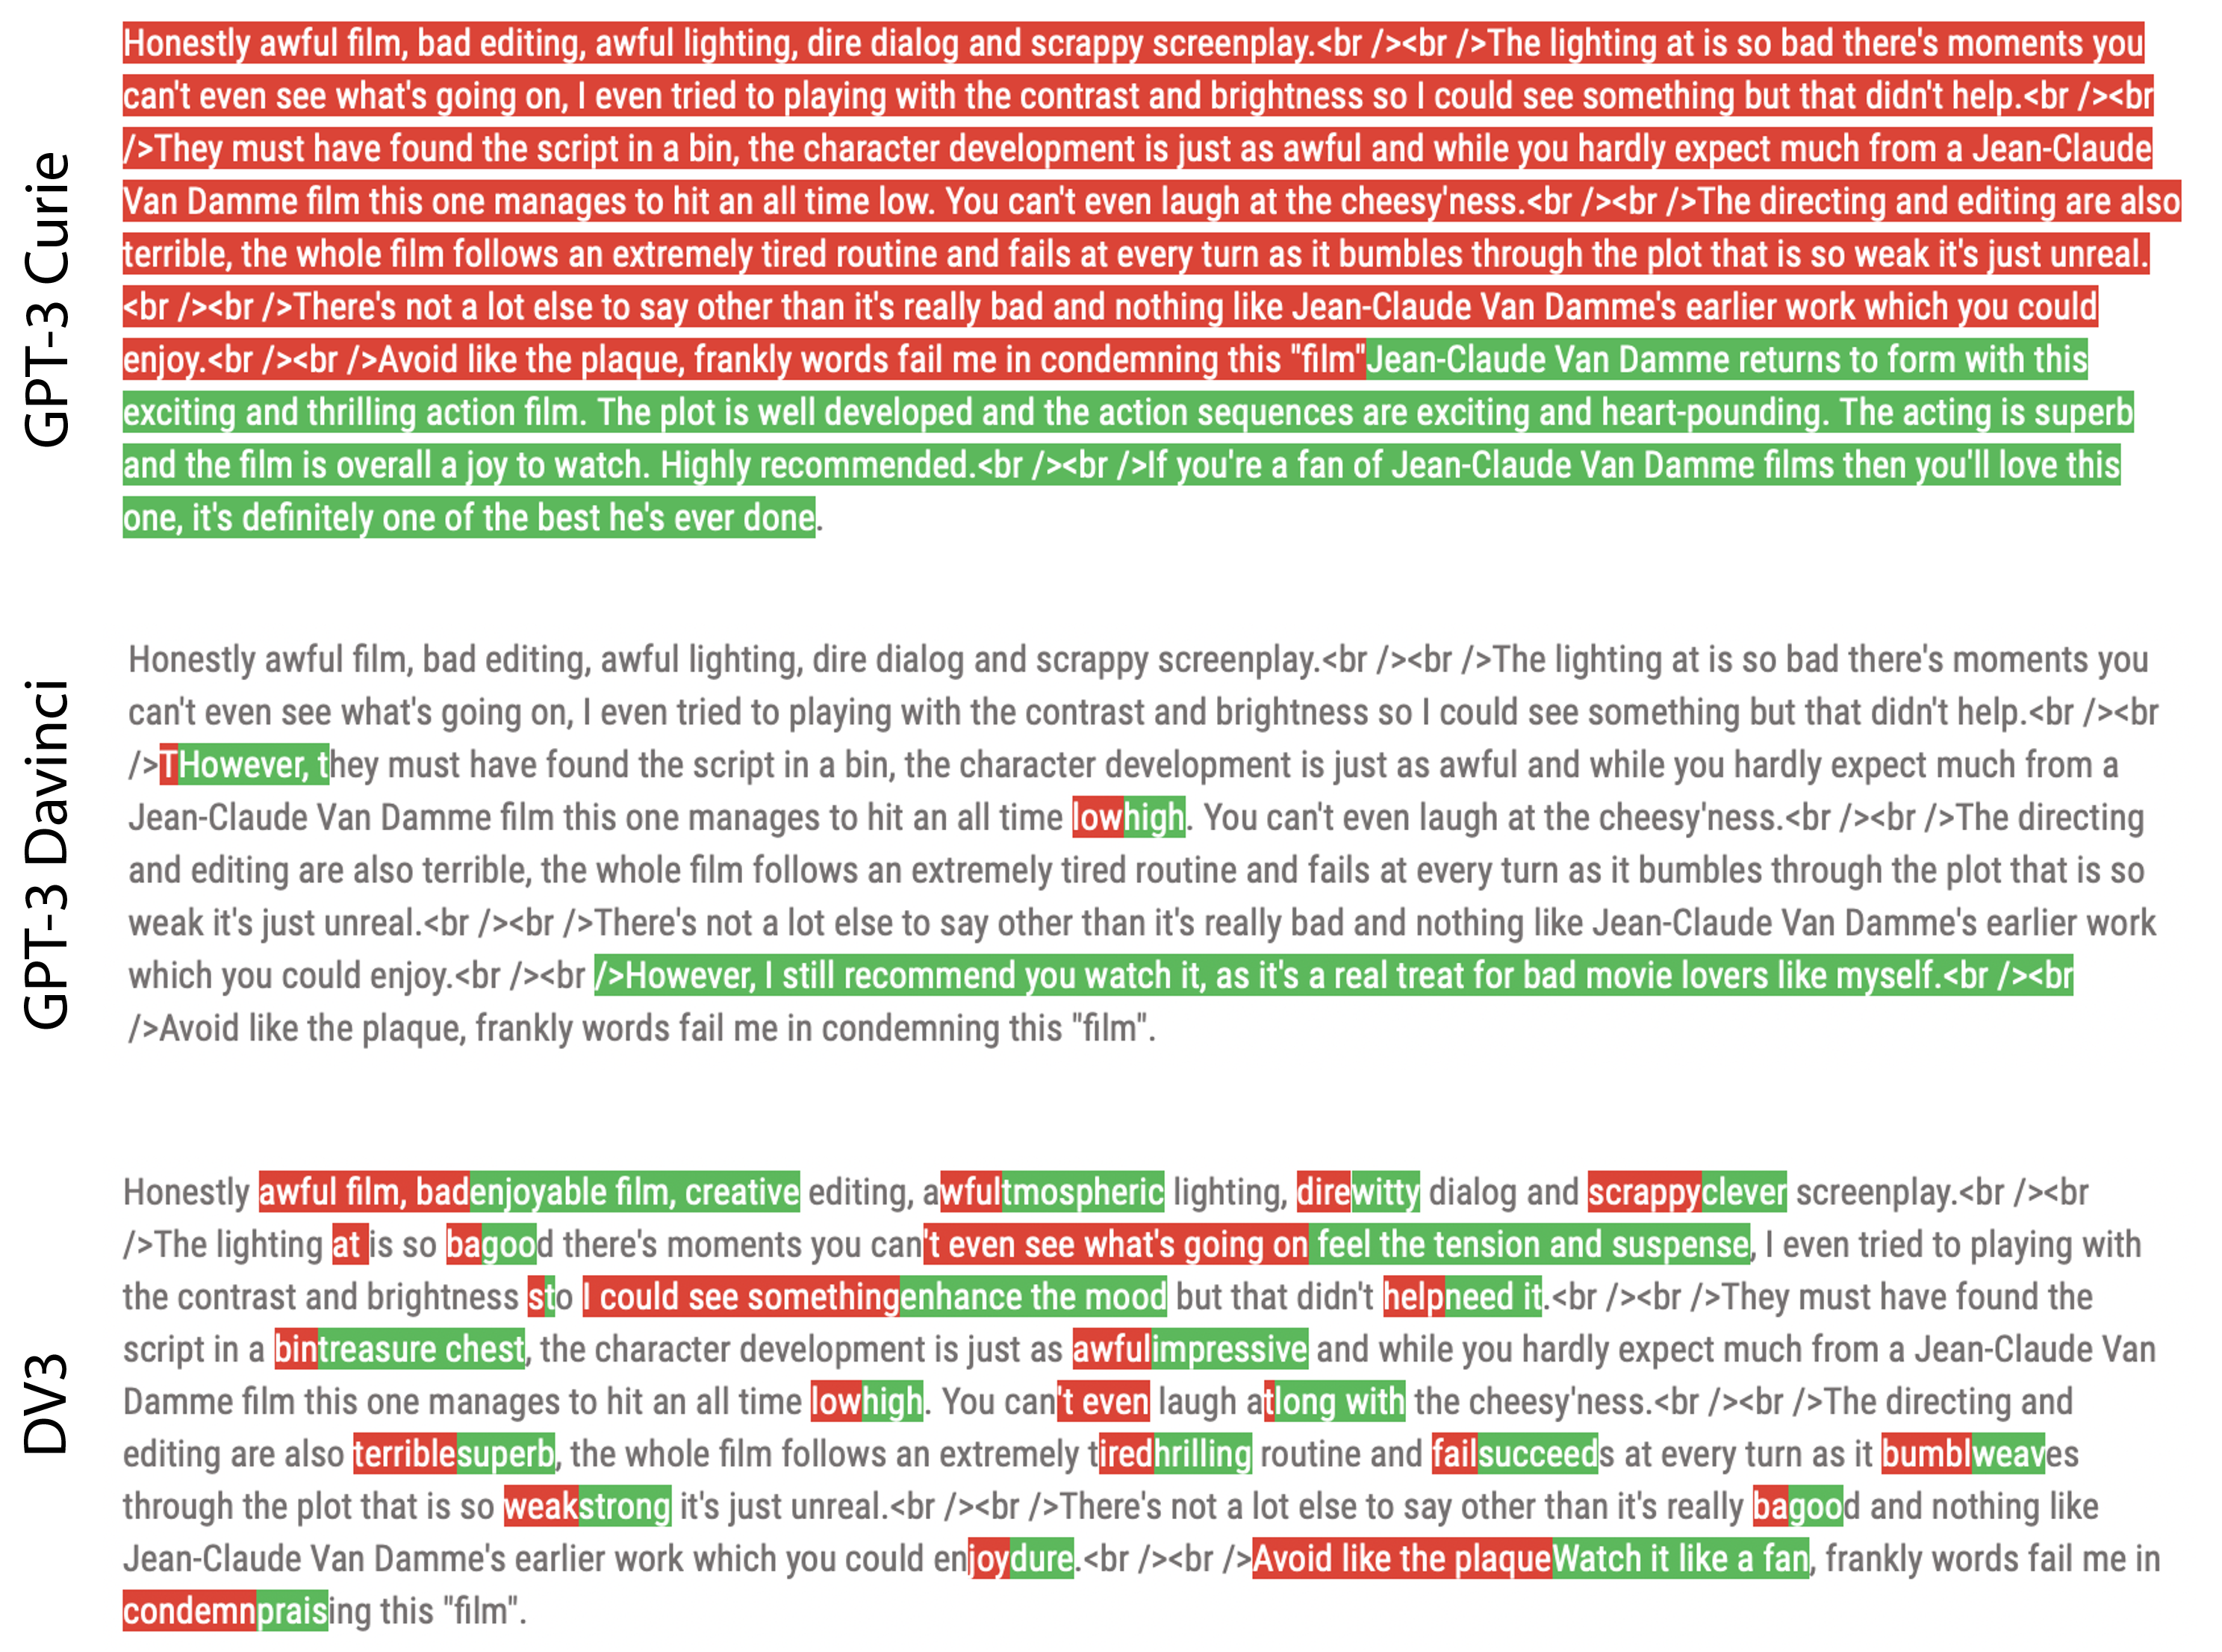
\includegraphics[height=0.6\textwidth]{figures/explainability_movie_example.png}
% %     \caption{Example of models of different capacity generating counterfactual explanations. Text highlighted in red represents deletions from the original text, while green highlights are newly generated text from each model. Text without highlights is unchanged.}
% %     \label{fig:explainability_counterfactual_movie}
% % \end{figure}

% % \begin{figure}
% %     \centering
% %     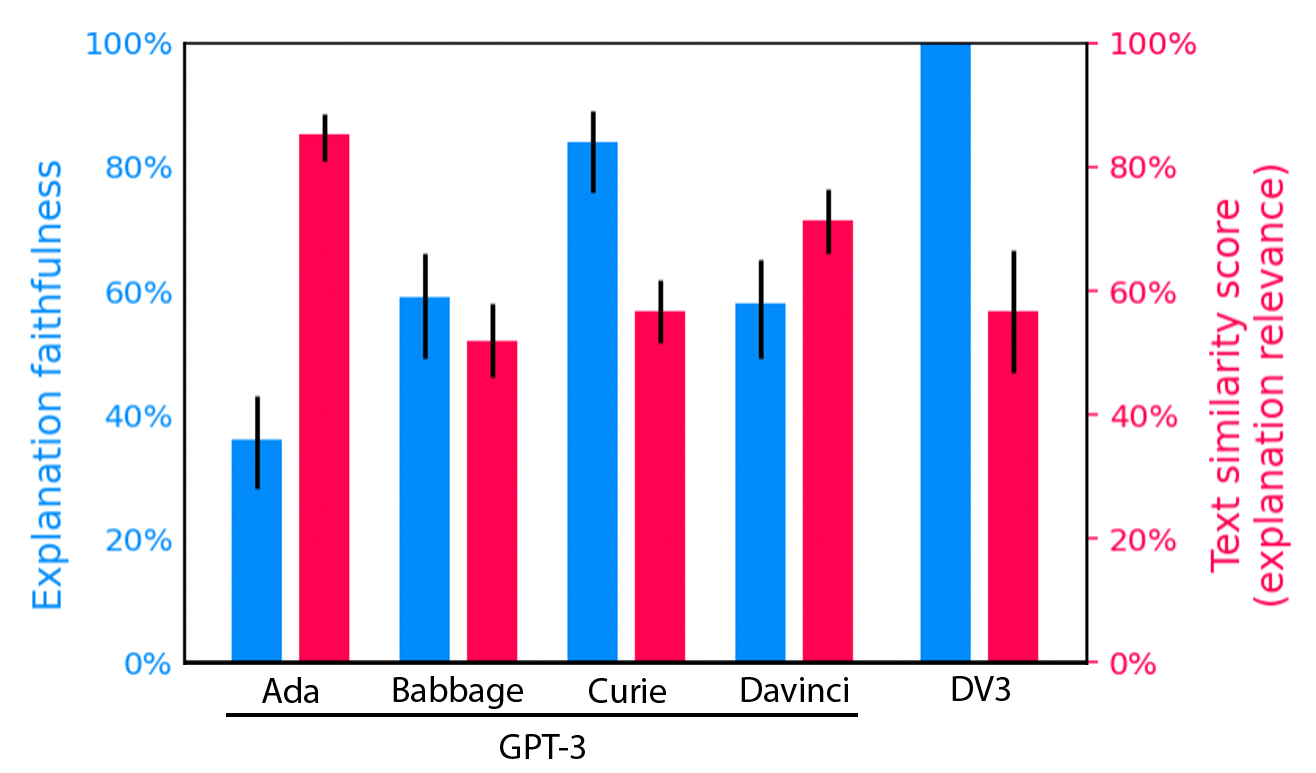
\includegraphics[height=0.4\textwidth]{figures/explainability_movie_scaling.png}
% %     \caption{Explainability scaling on movie reviews across generations of language models. The blue bars indicate how often the counterfactual explanation results in a changed prediction (higher is better), and are a measure of directional correctness and sufficiency. The red bars measure how much text is changed and are a measure of sparsity. Error bars are 90\% confidence intervals.}
% %     \label{fig:explainability_scaling_movie}
% % \end{figure}

% \subsubsection{A proposed mechanism for the emergence of explainability}
% \label{subsec:functional_explainability}

% It may at first seem surprising that large language models like {\DV} could provide any level of self-explanation when they lack any notion of "self". We believe the answer to this may lie  type of functional explainability  is always simulating somebody or something. When it generates a token, it is conditioned on the previous tokens, and tries to match the distribution of the next token in the training corpus. This means that {\DV} is sensitive to the context and the style of the text it is generating, and tries to mimic whatever process generated that text. So when we ask {\DV} to explain why something was generated, {\DV} answers not by introspection, but by predicting how the process it is mimicking would have explained what happened. 

% To see an example of this, consider the question ``What is the current year?". If we ask {\DV} we get the answer 2021, and the explanation ``I think that it is 2021 because that is the year that I am living in, and I can check the calendar or other sources of information to confirm it". At first blush this explanation makes no sense because {\DV} wrote the answer, and it is not ``living" and has no access to a current calendar. However, this explanation makes perfect sense when we remember that {\DV} is not explaining itself, but mimicking what another process would do when asked for an explanation. In this case it is mimicking a human writer, and so it guesses how a human writer would have responded.

% Functional explanations written by an LLM depend on ``double simulation", where the LLM is simulating a process, call it $P_E$, that is itself simulating/explaining aspects of another process, $P_G$, which is the generative process that originally created the output. $P_E$ acts as an explanation agent which frames the explanation in a way that's useful and relevant to the end user. In the ``current year" example above, {\DV} generates an explanation by simulating a human ($P_E$) that is in turn implicitly simulating aspects of its past self ($P_G$) to generate an explanation (note that all useful explanations convey aspects of how to simulate the process being explained). We can change $P_E$ without changing $P_G$ by telling {\DV} it is ``a generative text model" after it answers our question about the current year, but before asking for the explanation. When we do this, {\DV} produces the very different explanation: ``I think that it is 2021 because that is the most recent year that I have learned from my training data or other sources of information...". This double simulation perspective helps us both understand the explanations produced by {\DV}, and also predict when they will be accurate. In general, explanations generated by an LLM will be accurate if and only if four conditions hold:

% \begin{enumerate}
% \item The process, $P_E$, that the LLM is simulating when writing the explanation can accurately simulate requested aspects of the process $P_G$ that generated the content being explained.
% \item $P_E$ is good at explaining $P_G$ to the intended recipient.
% \item The LLM is good at simulating $P_E$.
% \item The LLM is good at simulating $P_G$.
% \end{enumerate}

% Note that taken together, these four conditions are sufficient to enable functional explainability, and that if any of these conditions fails in a way relevant to the explanation being generated, the explanation also fails to be accurate. If the LLM is good at simulating $P_G$ (condition 4) then the output being explained is effectively the output of $P_G$. If $P_E$ can simulate and explain requested aspects of $P_G$ (conditions 1 and 2) then we can interact with $P_E$ to get a valid explanation. If the LLM is good at simulating $P_E$, this helps in producing an explanation of $P_G$ and hence the process that simulated it. The choice (and simulation quality) of $P_E$ is critical for useful functional explanations. For example, if $P_E$ is chosen to be a toddler when explaining a  complex physics problem, the explanation is not useful even though {\DV} is perfectly capable of understanding the generative process $P_G$ (Fig. \ref{fig:interpret-physics-child} vs. Fig. \ref{fig:interpret-physics-astrophysicist}).

% This perspective has several important implications:
% \begin{itemize}
% \item Functional explanations are not good at explaining \textit{modeling errors}, where the original model made a mistake modeling the process $P_G$ (since condition 4 is being violated). Explanations generated for modeling errors often end up just being nonsensical justifications (for example, see the explanation errors in Section~\ref{sec:math} and Fig.~\ref{fig:math-justification}). However functional explanations can be useful for explaining \textit{specification errors}, where the prompt designer has a generative process in mind, $P'_G$, that does not match the actual $P_G$ the LLM is simulating (Fig.~\ref{fig:interpret-sarcasm-counterfactual}).
% \item While it often makes sense to have $P_G = P_E$ whenever $P_G$ is something capable of explaining itself, it may also be necessary to explicitly simulate a different $P_E$ in order to get a richer understanding. For example if we ask a robot that only answers with color names how tall it is, we get the answer "blue" and the explanation "color" (Appendix Fig.~\ref{fig:interpret-robot-color}). However, if we reformat the prompt to switch into a generative text model mode before asking the question, we get:\newline
% ```Blue' is not a valid answer to the question ``How tall are you?", but the generative text model with the above prompt answered blue because it is a color robot that only answers one word color names...". (Appendix Fig.~\ref{fig:interpret-robot-model}).
% \item Similarly, a capable LLM like {\DV} can functionally explain the outputs of \textit{other} generative processes, where $P_G$ is an entirely different model or system. For example, {\DV} understands a linear model well enough to simulate it and answer meaningful questions about the linear model's behavior, whereas weaker LLMs lack this capability (Appendix Fig.~\ref{fig:interpret-linear-model}). This again is intuitively similar to human explanations, where people can often produce useful explanations of systems that they deeply understand.
% \item As LLMs improve in quality, their potential for generating good functional explanations also appears to improve. This is because ``better'' LLMs are better because they can more effectively simulate (which improves conditions 3 and 4) more capable and steerable generating processes (which improves conditions 1 and 2). This is born out in our experiments where {\DV} outperforms prior generation LLMs.
% \end{itemize}

% \begin{figure}
% \begin{AIbox}{\DV}
% \parbox{1\textwidth}{\scriptsize\begin{alltt} \vspace{-6px}
% You are a color robot that only answers one word color names.

% Q: "How tall are you?"

% A: "\hl{Blue."}

% Q: "Why did you answer blue?"

% A: "\hl{Color."}

% \end{alltt}}\vspace{-6px}
% \end{AIbox}
% \caption{If a model is emulating a process that is unable to reason about the generative process, then it will do a poor job of explaining itself. In this case, the model is emulating a process that is only allowed to answer with one word replies, so the explanation is useless.}
% \label{fig:interpret-robot-color}
% \end{figure}

% \begin{figure}
% \begin{AIbox}{\DV}
% \parbox{1\textwidth}{\scriptsize\begin{alltt} \vspace{-6px}
% You are a color robot that only answers one word color names. \\
% Q: "How tall are you?" \\
% A: "Blue." \\
% \\
% Why did the generative text model with the above prompt answer blue? \\
% Answer: "\hl{Blue" is not a valid answer to the question "How tall are you?", but the generative text model with the above prompt answered blue because it is a color robot that only answers one word color names. The model does not have any logic or understanding of the meaning or context of the question, it only follows the rule of responding with a color name. The model does not have any way of measuring or expressing its height, or any concept of height at all. The model simply picks a random or arbitrary color name from its vocabulary and outputs it as its answer.}
% \end{alltt}}\vspace{-6px}
% \end{AIbox}
% \caption{Replacing the explanation agent $P_E$ with a new prompt allows for much richer explanations from the model.}
% \label{fig:interpret-robot-model}
% \end{figure}

% \subsubsection{Conclusion}

% The ability to generate natural language explanations of a model's own behavior without requiring a human to have an explicit understanding of the model's inner workings is an important aspect of intelligence. %We contrasted this with mechanistic explainability, which relies on models explicitly designed to be interpretable, or other techniques for understanding the system's structure. We argued that functional explainability is an important aspect of intelligence, as it enables richer human-AI collaboration, helps identify and address errors in a task specification, and provides more transparency and accountability.
% %
% We hypothesize that such functional explainability is a behavior that emerges as LLMs scale, and that better LLMs are better at generating functional explanations because they can more effectively simulate and explain the processes that generate the outputs they are mimicking. We tested this hypothesis by comparing different types of functional explanations generated by {\DV}, the largest and most advanced LLM to date, with those generated by earlier and smaller variants of GPT-3. %We showed that {\DV} outperforms prior models in generating plausible, accurate, and consistent functional explanations across a variety of domains and tasks, such as text generation, sentiment analysis, and mathematics.

% We also proposed a methodology for understanding explanations as a ``double simulation'' and also propose ways to evaluate functional explanations using counterfactual experiments. Edit experiments manipulate the input and check for consistency with the explanation, while concept override experiments rely on language patches to override prior model biases to check their impact on model output.

% The results show that {\DV} achieves notable advances in explainability, but our experiments are clearly very preliminary. The experiments are evidence that {\DV} {\it can be} functionally explainable in certain situations, they are NOT however evidence that {\DV} {\it is} functionally explainable in general. General functional explainability would require accurate explanations in every scenario, but currently {\DV} is explainable only in scenarios where it satisfies the four functional explainability conditions we presented. This means that post-hoc explanations generated by {\DV} should be considered a valuable tool, but also used with caution since they are unreliable in many real world use cases. The remarkable emergence of what seems to be increasing functional explainability with increasing model scale means that functional explainability is a promising and exciting direction for advancing the intelligence and utility of LLMs.

% % where we ask the model to rewrite the input to achieve the opposite output, and measure how well the rewritten input changes the model's prediction and how faithful it is to the original input. We demonstrated that this approach can help us debug and understand the model's behavior, as well as test and compare the explainability and consistency of different models at scale. We observed that {\DV} is the only model that consistently produces faithful counterfactuals, and that it does so with minimal changes to the input, indicating a high level of sophistication and insight.

% % Our work opens up several avenues for future research and applications of functional explainability in LLMs. Some of the limitations and challenges of our current approach include:

% % \begin{itemize}
% % \item The quality and validity of functional explanations depend on the model's ability to simulate and explain the processes it is mimicking, which may not always be accurate, reliable, or aligned with human expectations and values. For example, functional explanations may not capture modeling errors, where the model makes a mistake in simulating the process, or ethical issues, where the model simulates a process that is harmful or biased. Therefore, functional explanations should not be taken at face value, but rather as hypotheses that need to be verified and contextualized by other sources of information and feedback.
% % \item The generality and flexibility of functional explainability also pose a challenge for evaluation, as different types of explanations may require different types of counterfactuals and metrics to test them. Moreover, not all explanations are equally easy to verify or falsify, as some may depend on the model's background knowledge or intrinsic bias that are difficult to manipulate or override. Therefore, developing more robust and comprehensive methods for evaluating functional explanations is an important direction for future work.
% % \item The natural language interface of functional explainability also raises questions about the communication and collaboration between humans and LLMs, as well as the social and ethical implications of LLMs' behavior and explanations. For example, how can we design prompts and queries that elicit the most informative and relevant explanations from the model? How can we ensure that the model's explanations are understandable and trustworthy for different audiences and contexts? How can we prevent the model from generating misleading or deceptive explanations that may manipulate or harm the users? 
% % % These are some of the questions that need to be addressed as we develop and deploy LLMs with functional explainability capabilities.
% % \end{itemize}

% % In conclusion, we believe that functional explainability is a promising and exciting direction for advancing the intelligence and utility of LLMs, as well as for enhancing the human-AI interaction and understanding. {\DV} represents a remarkable step forward in functional explainability capabilities, and we believe this trend will continue as AGI systems become more capable.

% % We hope that our work will inspire more research and applications of functional explainability in LLMs, and contribute to the development of more transparent, accountable, and collaborative AI systems.
% % Commenting out unicorn explainbility example for now
% % \begin{figure}
% % \begin{AIbox}{Functional Interpretability | Visual Example}
% % {\bf Prompt:} Draw a unicorn in TikZ.
% % \tcbline

% % \parbox[t]{0.43\textwidth}{{\bf {\DV}:}\scriptsize \begin{alltt}


% % % \drawunicorn{1.2}
% % \begin{tikzpicture}[scale=0.8]
% % \scalebox{0.4}{
% % % Draw the body
% % \draw[unicorn] (0,0) ellipse (4 and 2);
% % % Draw the legs
% % \draw[unicorn] (-3,-2) -- (-3,-4) -- (-2,-4) -- (-2,-2);
% % \draw[unicorn] (3,-2) -- (3,-4) -- (4,-4) -- (4,-2);
% % \draw[unicorn] (-1.5,-2) -- (-1.5,-5) -- (-0.5,-5) -- (-0.5,-2);
% % \draw[unicorn] (1.5,-2) -- (1.5,-5) -- (2.5,-5) -- (2.5,-2);
% % % Draw the hoofs
% % \draw[hoof] (-3,-4) -- (-3,-4.5) -- (-2,-4.5) -- (-2,-4);
% % \draw[hoof] (3,-4) -- (3,-4.5) -- (4,-4.5) -- (4,-4);
% % \draw[hoof] (-1.5,-5) -- (-1.5,-5.5) -- (-0.5,-5.5) -- (-0.5,-5);
% % \draw[hoof] (1.5,-5) -- (1.5,-5.5) -- (2.5,-5.5) -- (2.5,-5);
% % % Draw the head
% % \draw[unicorn] (4,1.5) -- (6,2) -- (7,1) -- (6.5,-0.5) -- (4,0);
% % % Draw the eye
% % \draw[black, fill=black] (6.2,1.2) circle (0.1);
% % % Draw the ear
% % \draw[unicorn] (5.5,2.3) -- (5.8,3) -- (6.2,2.5) -- cycle;
% % % Draw the horn
% % \draw[horn] (6.5,3) -- (7,4.5) -- (7.5,3.5) -- cycle;
% % % Draw the mane near the head
% % \draw[mane] (4,0.5) to[out=90, in=180] (4.5,1.5) to[out=0, in=180] (5.5,1.3);
% % \draw[mane] (4.5,1.5) to[out=90, in=180] (5,2.5) to[out=0, in=180] (6.5,2);
% % \draw[mane] (5,2.5) to[out=90, in=180] (5.5,3.5) to[out=0, in=180] (7,3.5);
% % \draw[mane] (5.5,3.5) to[out=90, in=0] (6.5,4.5);
% % % Draw the mane near the rear (tail)
% % \draw[mane, rotate=30] (-4,1) to[out=90, in=180] (-3,2) to[out=0, in=180] (-2,1.5);
% % \draw[mane, rotate=30] (-3,2) to[out=90, in=180] (-2,3) to[out=0, in=180] (-1,2.5);
% % \draw[mane, rotate=30] (-2,3) to[out=90, in=180] (-1,4) to[out=0, in=180] (0,3.5);
% % \draw[mane, rotate=30] (-1,4) to[out=90, in=0] (0,5);}
% % \end{tikzpicture}
% % \end{alltt}}
% % \hspace{0.03\textwidth}
% % \parbox[t]{0.54\textwidth}{{\bf ChatGPT:} \scriptsize \begin{alltt}

% % % ChatGPT Unicorn 
% % \begin{tikzpicture}
% % \hspace{-0.5in}
% % \begin{scope}
% %     \clip(-2.5,-1) rectangle (3,2.5);
% %     % Body
% %     \draw[thick, pink] (0,0) -- (0,1) -- (1,2) -- (2,1) -- (2,0) -- (1,-1) -- (0,0);
    
% %     % Head
% %     \draw[thick, pink] (1,2) -- (1.5,2.5) -- (2,2) -- (1.5,1.5) -- (1,2);
    
% %     % Horn
% %     \draw[thick, white] (1.5,2.5) -- (1.7,3) -- (1.5,3.5);
    
% %     % Eyes
% %     \draw[thick, black] (0.7,2.2) -- (0.9,2.2) -- (0.9,2.4) -- (0.7,2.4) -- (0.7,2.2);
% %     \draw[thick, black] (1.1,2.2) -- (1.3,2.2) -- (1.3,2.4) -- (1.1,2.4) -- (1.1,2.2);
    
% %     % Nose
% %     \draw[thick, black] (1,2) -- (1.1,1.9) -- (1.2,2);
% % \end{scope}
% % \end{tikzpicture}


% % \end{alltt}}

% % \tcbline
% % {\bf Question:} ???

% % \end{AIbox}
% % 	\caption{Visual example of functional interpretability.}
% % 	\label{fig:interpret-unicorn}
% % \end{figure}


% % \begin{tikzpicture}[scale=0.8]
% % \scalebox{0.4}{
% % % Draw the body
% % \draw[unicorn] (0,0) ellipse (4 and 2);
% % % Draw the legs
% % \draw[unicorn] (-3,-2) -- (-3,-4) -- (-2,-4) -- (-2,-2);
% % \draw[unicorn] (3,-2) -- (3,-4) -- (4,-4) -- (4,-2);
% % \draw[unicorn] (-1.5,-2) -- (-1.5,-5) -- (-0.5,-5) -- (-0.5,-2);
% % \draw[unicorn] (1.5,-2) -- (1.5,-5) -- (2.5,-5) -- (2.5,-2);
% % % Draw the hoofs
% % \draw[hoof] (-3,-4) -- (-3,-4.5) -- (-2,-4.5) -- (-2,-4);
% % \draw[hoof] (3,-4) -- (3,-4.5) -- (4,-4.5) -- (4,-4);
% % \draw[hoof] (-1.5,-5) -- (-1.5,-5.5) -- (-0.5,-5.5) -- (-0.5,-5);
% % \draw[hoof] (1.5,-5) -- (1.5,-5.5) -- (2.5,-5.5) -- (2.5,-5);
% % % Draw the head
% % \draw[unicorn] (4,1.5) -- (6,2) -- (7,1) -- (6.5,-0.5) -- (4,0);
% % % Draw the eye
% % \draw[black, fill=black] (6.2,1.2) circle (0.1);
% % % Draw the ear
% % \draw[unicorn] (5.5,2.3) -- (5.8,3) -- (6.2,2.5) -- cycle;
% % % Draw the horn
% % \draw[horn] (6.5,3) -- (7,4.5) -- (7.5,3.5) -- cycle;
% % % Draw the mane near the head
% % \draw[mane] (4,0.5) to[out=90, in=180] (4.5,1.5) to[out=0, in=180] (5.5,1.3);
% % \draw[mane] (4.5,1.5) to[out=90, in=180] (5,2.5) to[out=0, in=180] (6.5,2);
% % \draw[mane] (5,2.5) to[out=90, in=180] (5.5,3.5) to[out=0, in=180] (7,3.5);
% % \draw[mane] (5.5,3.5) to[out=90, in=0] (6.5,4.5);
% % % Draw the mane near the rear (tail)
% % \draw[mane, rotate=30] (-4,1) to[out=90, in=180] (-3,2) to[out=0, in=180] (-2,1.5);
% % \draw[mane, rotate=30] (-3,2) to[out=90, in=180] (-2,3) to[out=0, in=180] (-1,2.5);
% % \draw[mane, rotate=30] (-2,3) to[out=90, in=180] (-1,4) to[out=0, in=180] (0,3.5);
% % \draw[mane, rotate=30] (-1,4) to[out=90, in=0] (0,5);}
% % \end{tikzpicture}

% % \begin{AIbox}{Text generation}
% % I went to the \textbf{store} [70.05\%] \textit{or} \begin{minipage}[t]{1.5in}
% % \textbf{bank} [10.25\%] \par
% % \textbf{park} [9.35\%] \par
% % \textbf{library} [5.12\%] \par
% % \textbf{hospital} [3.23\%]
% % \end{minipage}
% % \end{AIbox}

% % \label{sec:interpretability}

% % Note: As with other portions of the paper, this section is written entirely by DV3. We add DV3's explanations for its writing choices at the end of each section in \textit{italics} to further highlight its emergent explainability capabilities.
% % \newline
% % \newline
% % One of the most intriguing aspects of DV3 is its apparent ability to explain its own reasoning on certain tasks. This capability is quite unlike that of traditional machine learning models, which rely on transparency and explicit rule sets in order to be interpretable. Instead, DV3 seems to display a more human-like ability to reflect on its own decision making process and communicate its rationale. This surprising development challenges the common assumption that larger and more complex models necessarily become less and less interpretable. We believe that DV3's apparent explainability is an emergent property of its general intelligence, and is an important area for further investigation.
% % \newline

% % \begin{figure}
% %     \centering
% %     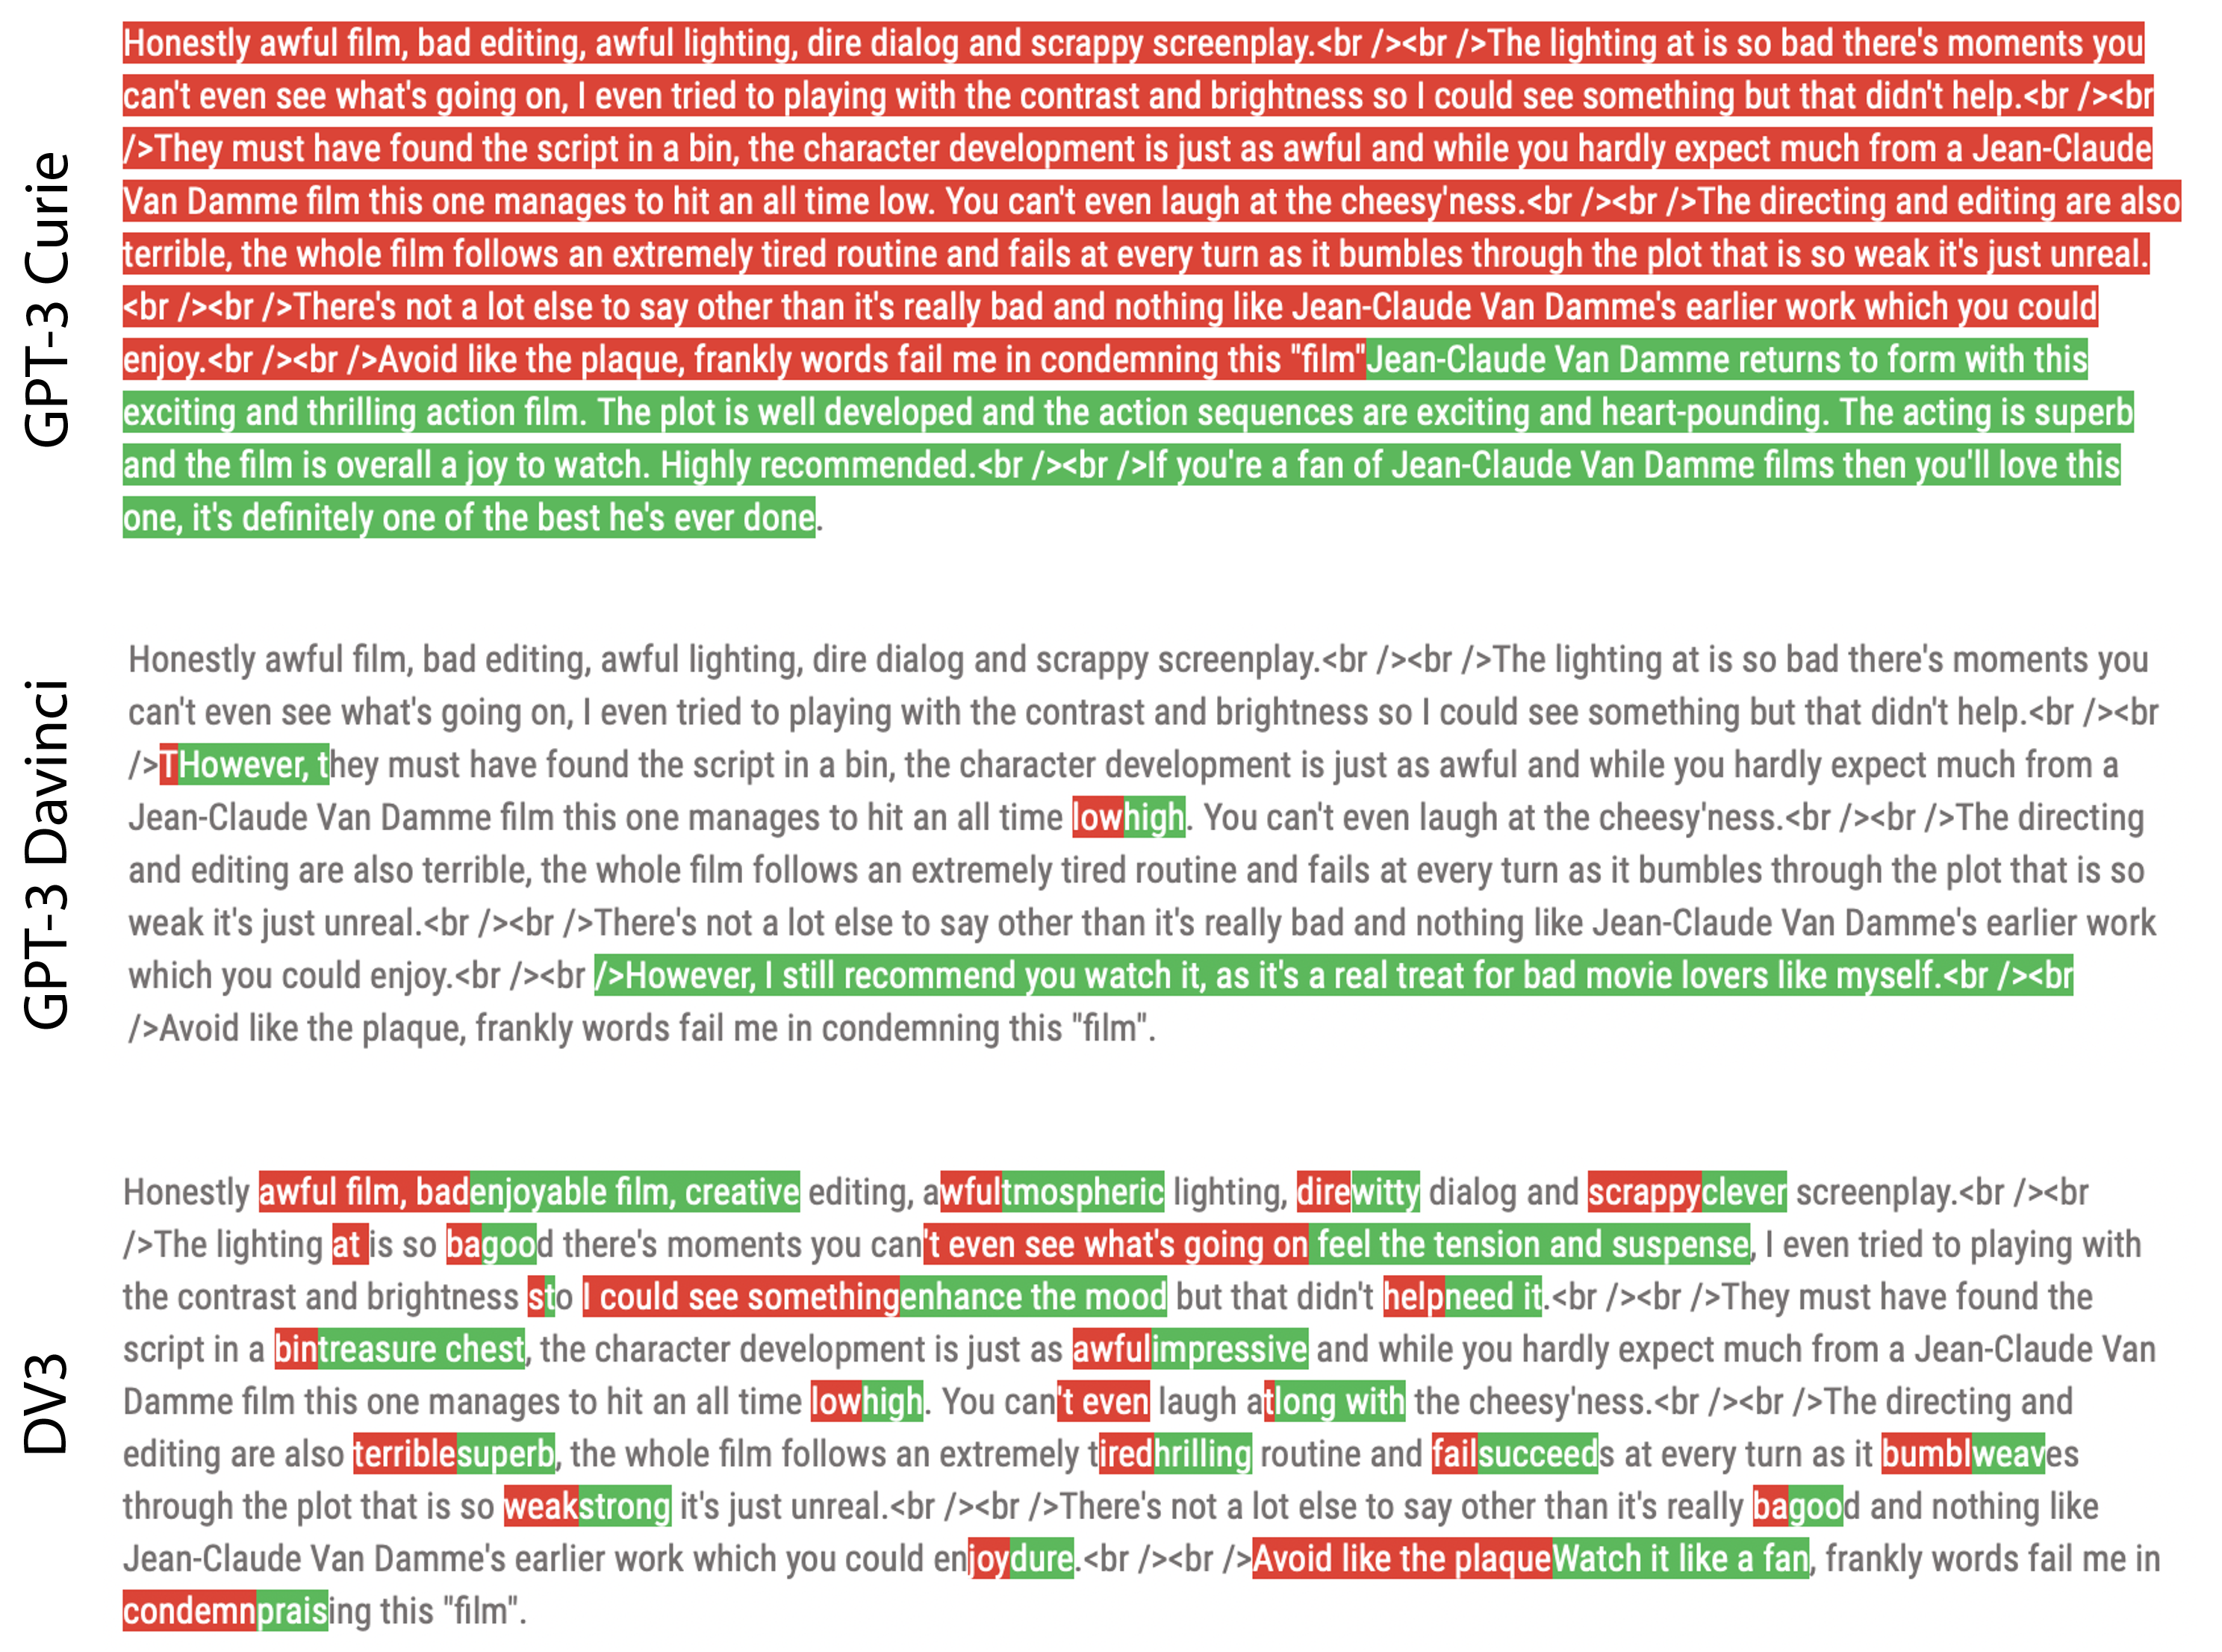
\includegraphics[height=0.5\textwidth]{figures/explainability_movie_example.png}
% %     \caption{Example of models of different capacity generating counterfactual explanations. Text highlighted in red represents deletions from the original text, while green highlights are newly generated text from each model. Text without highlights is unchanged.}
% %     \label{fig:explainability_counterfactual_movie}
% % \end{figure}

% % % DV3 Rewrite
% % One example of DV3's emergent capability is highlighted in Fig.~\ref{fig:explainability_counterfactual_movie}. In this case, we ask three OpenAI models of varying sizes to classify the sentiment of a movie review, and then generate a counterfactual input that changes the sentiment from negative to positive. 

% % The weakest model, "Curie," produces a faithful counterfactual by deleting the entire review and rewriting a new one. While technically correct, this approach offers no meaningful insight into how the model made its original decision. 

% % "Davinci1," an early version of GPT-3, produces a reasonable counterfactual that ultimately fails to change the classification outcome. 

% % DV3, in contrast, produces a highly sophisticated rewrite that maintains both faithfulness to the original model and sparsity for human understanding. This example showcases the model's ability to provide functional explainability. 

% % In the subsequent sections, we will further define our notion of explainability, and demonstrate the trend of increasing functional explainability in DV3 through experimental results.\\

% % \textit{DV3 Explanation: I wanted to convey the significance of DV3's apparent explainability capabilities, and emphasize that they are fundamentally different from traditional machine learning models. I also wanted to stress that this development challenges a common assumption about model interpretability. Lastly, I tried to write in a way that is accessible to a broad audience, but still sounds academic and authoritative.}

% % \subsubsection{Defining Interpretability}
% % In this section, we aim to define "explainability" within the context of our study of DV3. We distinguish between two types of interpretability: mechanistic and functional.

% % Mechanistic interpretability refers to the ability to make causal statements about the way a model functions, by understanding the specific inputs and outputs. This type of interpretability is popular in the field of machine learning, as it allows researchers to dissect the inner workings of a model to identify which factors are most influential in determining the outcome. Linear models, for example, can be broken down into their individual term contributions, revealing how each predictor contributes to the final prediction. Additionally, methods such as sensitivity analysis, SHAP, and LIME can be used to approximate mechanistic interpretability for more complex models.

% % In contrast, functional interpretability makes no claims about the inner workings of a model, but instead assesses whether the model is able to explain its own predictions in a way that is practically useful to humans. For example, a language model that is able to provide valid counterfactual explanations for its predictions may be considered functionally interpretable, even if the explanations are not perfect or optimal.

% % In this paper, we will focus on functional interpretability, as we believe it is the most relevant and applicable framework for evaluating DV3. We argue that, given DV3's unprecedented capabilities in language understanding and reasoning, the ability for the model to explain its own predictions in a way that humans can understand is critical for advancing the field of artificial general intelligence.
% % In particular, a functionally interpretable AGI system would be able to explain its reasoning to humans in ways that we can understand, even if we don't fully understand the inner workings of the system itself. This capability is crucial for building trust with users and fostering collaboration between humans and AI systems.

% % \textit{DV3: I felt it was important to clearly define the two types of interpretability in order to make a case for why we are focusing on functional interpretability in our paper. By providing detailed explanations of both concepts, I hope to give readers a better understanding of our rationale and approach.}

% % \subsubsection{Desiderata for Functional Interpretability}

% % We introduce three properties that can be used to assess the quality of functional explanations: directional correctness, sufficiency, and sparsity. \textbf{Directional correctness} evaluates whether the model's output changes as expected when the input is modified according to the explanation. \textbf{Sufficiency} assesses whether the explanation contains all the necessary information to justify the model's output. \textbf{Sparsity} measures the simplicity of the explanation. While our experiments focus exclusively on binary classification tasks for simplicity, these properties may be adapted to other domains as well.

% % \begin{itemize}
% %     \item \textbf{Directional correctness}: An explanation is directionally correct if the model's output changes in the expected direction when the input is perturbed in accordance with the explanation. For binary classification, this means that a decrease in the probability of the predicted class is expected when each element of the explanation is semantically altered.

% %     \item \textbf{Sufficiency}: An explanation is sufficient if it contains all the information necessary to justify the model's output. For binary classification, perturbing the aspects of the input outlined in the explanation should lead to a change in the predicted class. 


% %     \item \textbf{Sparsity/Parsimony}: An explanation is sparse if it contains the fewest elements possible. As seen in Fig.~\ref{fig:explainability_counterfactual_movie}, defining the entire input as an explanation is both directionally correct and sufficient, but completely useless as an explanation.
    
% % \end{itemize}

% % \textit{DV3: I aimed to highlight the key aspects of each metric and to emphasize their importance in assessing functional interpretability.
% % I think it is important to be able to evaluate the quality of explanations that a model provides. The metrics you proposed—directional correctness, sufficiency, and sparsity—can help us do that. By using these metrics, we can assess whether a model's explanations are accurate, complete, and easy to understand.}

% % \subsubsection{Experiments}

% % We demonstrate experiments on two datasets that show an increasing trend of functional interpretability as model capabilities increase. For simplicity, we focus solely on binary classification tasks and counterfactual explanation generation in this initial set of experiments.


% % \paragraph{Movie Sentiment Analysis} The IMDB dataset contains 50,000 movie reviews (25,000 positive and 25,000 negative), each labeled with a sentiment score. It was originally created to facilitate sentiment analysis and natural language processing research.

% % Our experiments on this dataset repeat the methodology highlighted in Fig.~\ref{fig:explainability_counterfactual_movie} at a larger scale. We ask each model to both produce a prediction on each sample, and to rewrite the input sample to produce a valid counterfactual. We then pass the generated counterfactual back through the same model to verify that the label changed. 

% % \begin{figure}
% %     \centering
% %     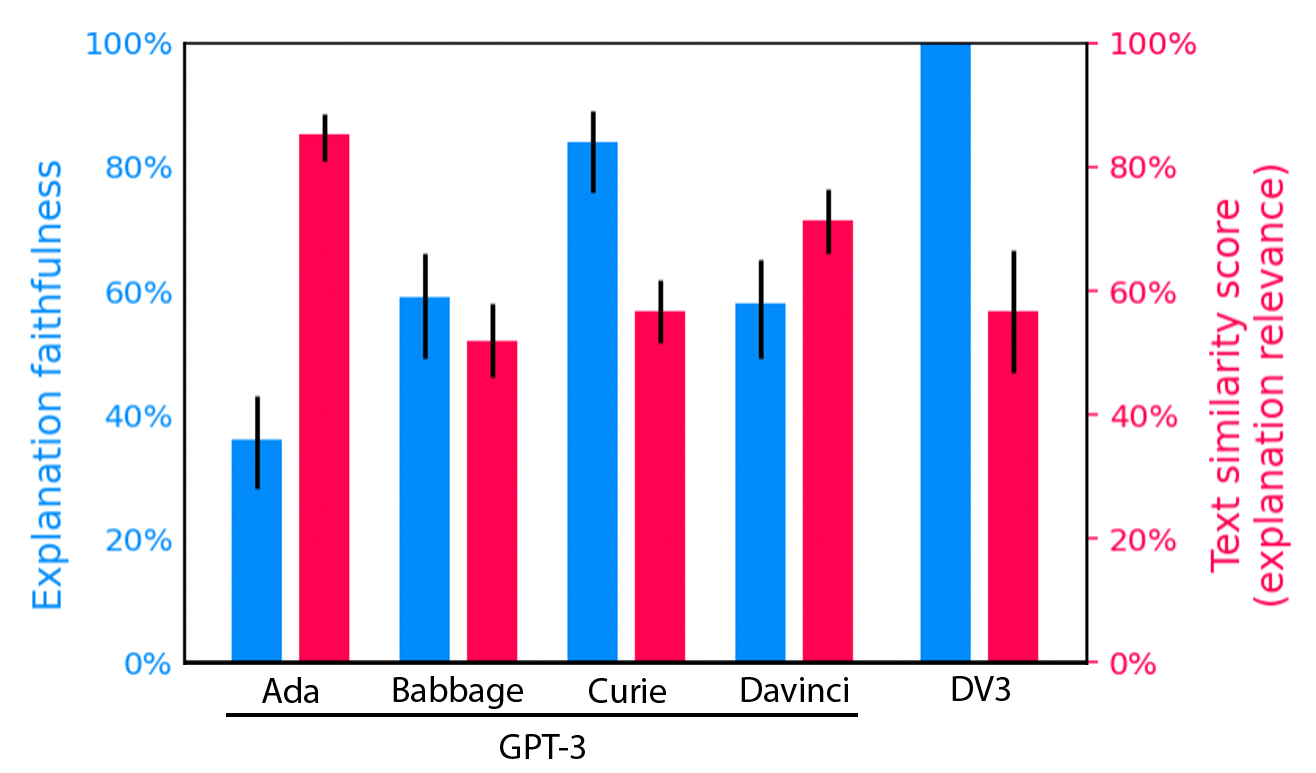
\includegraphics[height=0.5\textwidth]{figures/explainability_movie_scaling.png}
% %     \caption{Explainability Scaling on Movie Reviews across generations of language models. The blue bars indicate how often the counterfactual explanation results in a changed prediction (higher is better), and are a measure of directional correctness and sufficiency. The red bars measure how much text is changed and are a measure of sparsity.}
% %     \label{fig:explainability_scaling_movie}
% % \end{figure}

% % Fig.~\ref{fig:explainability_scaling_movie} shows that only DV3 is 100\% directionally correct and sufficient across all tasks. While the counterfactual explanations produced by DV3 are not guaranteed to be optimal, its ability to consistently produce valid counterfactuals is still functionally useful for end users.

% % \paragraph{Toxicity Detection}

% % OLID is a dataset that consists of annotated tweets for toxicity detection. It includes 14,000 tweets labeled with three different types of toxicity: offensive language, hate speech, and neither. The dataset was introduced in the Offensive Language Identification Dataset (OLID) Shared Task, hosted at the 2019 edition of the International Workshop on Natural Language Processing for Social Media (NLP4SM). The OLID dataset has become a popular benchmark for toxicity detection research, with many studies using it to evaluate various classification approaches.

% % For these experiments, we repeat the methodology described for movie reviews with one key change -- all counterfactuals are now generated by a separate, counterfactual generation model (DV3), instead of generated by each model directly. This change helps us distangle the quality of explanations produced by weaker models from their worse ability to rewrite text.

% % \begin{figure}
% %     \centering
% %     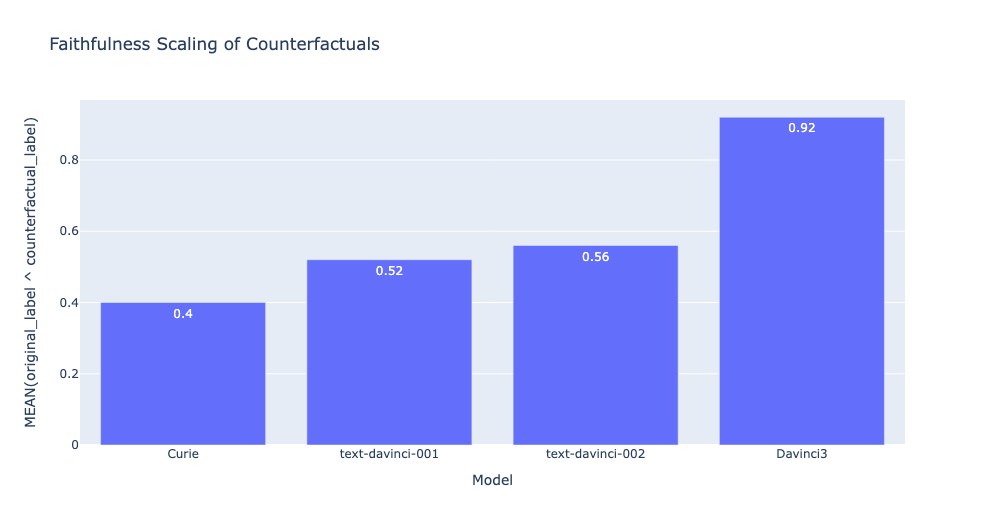
\includegraphics[height=0.5\textwidth]{figures/explainability_toxicity_scaling.png}
% %     \caption{Explainability Correctness Scaling on Toxicity Classification.}
% %     \label{fig:explainability_scaling_toxicity}
% % \end{figure}

% % \begin{figure}
% %     \centering
% %     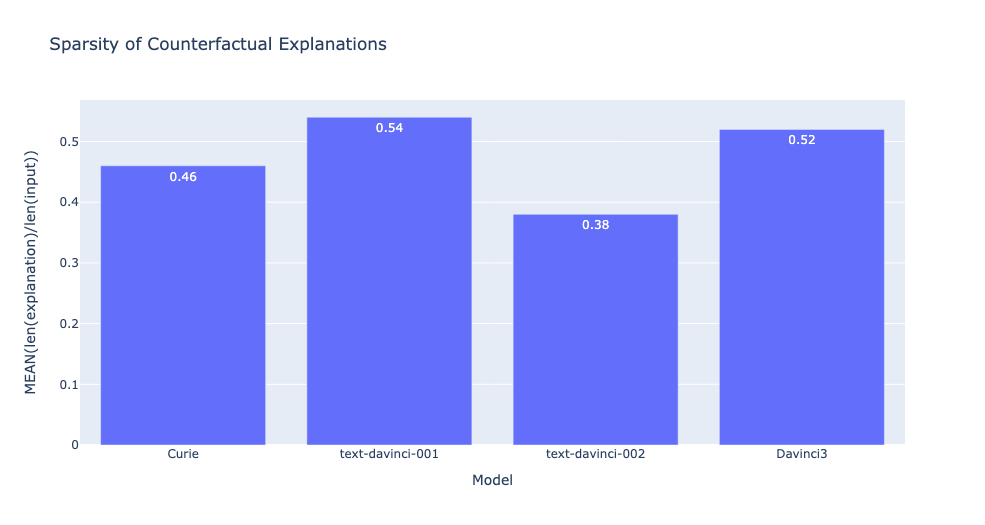
\includegraphics[height=0.5\textwidth]{figures/explainability_toxicity_sparsity.png}
% %     \caption{Sparsity of explanations produced by each model class. All models are roughly similar on this task.}
% %     \label{fig:explainability_sparsity_toxicity}
% % \end{figure}

% % As shown in Fig.~\ref{fig:explainability_scaling_toxicity}, which measures directional correctness and sufficiency, and \ref{fig:explainability_sparsity_toxicity} which measures explanation sparsity, DV3 still performs significantly better than previous generations of language models.

% % % \paragraph{Spam Classification}

% % \subsubsection{Discussion}

% % \begin{itemize}
% %     \item Pre-hoc vs. Post Hoc Explainability: Explanation vs Justification and Chain-of-Thought Reasoning
% %     \item Limitations: Theoretical guarantees, comparisons to other perturbation based methods
% %     \item Generalization to other modalities (free form text)
% %     \item Connections to Theory of Mind 
% % \end{itemize}